\documentclass[11pt,a4paper]{article}
\usepackage[margin=24mm]{geometry}
\usepackage{amsmath,amssymb,bm}
\usepackage{graphicx}
\usepackage{booktabs}
\usepackage{array}
\usepackage{enumitem}
\usepackage[hidelinks]{hyperref}
\usepackage{microtype}
\graphicspath{{../figures/}{../}}
\setlength{\parskip}{4pt}
\newcommand{\vect}[1]{\mathbf{#1}}
\newcommand{\code}[1]{\texttt{#1}}

\title{The aerodynamic model of the Vortex Step Method code\\[4pt]\large formulation, conventions and validation}
\author{Vortex-Step-Method repository, \code{docs/aerodynamic\_model/aerodynamic\_model.tex}}
\date{October 2026}

\begin{document}
\maketitle

\begin{abstract}
\noindent This document describes the aerodynamic model implemented in the Vortex-Step-Method (VSM) code as it stands in October 2026: a nonlinear lifting-line method in which an outer three-dimensional vortex system (bound vortex, attached-trailed legs, frozen semi-infinite wake) is coupled to an inner two-dimensional airfoil model (polars) with the consistent coupling rules of Gaunaa, Li and Pirrung (TORQUE 2026). It states every convention the results depend on, gives the equations as they are coded, and collects the validation: analytical wings, the Trefftz-plane consistency of the induced drag, a vortex-lattice referee on planar, swept, curved and kite-like wings, and the TU~Delft V3 kite against RANS and wind-tunnel data. It replaces the thesis chapter that this file used to hold. Each section names the code that implements it and the script that reproduces its figures.
\end{abstract}

\tableofcontents

\section{Scope and how to read this document}
\label{sec:scope}
The code computes the steady aerodynamic forces and moments on one or more thin lifting surfaces in a prescribed inflow, including rigid-body rotation rates and an inflow that varies along the span, with optional bridle lines. It is used for kite design, trim and stability analysis and as the aerodynamic module of fluid--structure couplings, where it must be fast (a kite with 50 panels solves in well under a second), robust on unconventional planforms (curved, swept, low aspect ratio) and free of three-dimensional empirical data. Potential-flow vortex methods meet these requirements; among them the lifting line with sectional polars is the fastest, and its known weaknesses on curved and swept wings are what the coupling rules of Section~\ref{sec:coupling} address.

Sections~\ref{sec:assumptions}--\ref{sec:solver} describe the model: assumptions, geometry and discretisation, the vortex system, the inner--outer coupling, and the solver with its outputs. Section~\ref{sec:validation} is the validation. Section~\ref{sec:conventions} is a table of conventions for people who read results. Every figure is generated by a script in \code{docs/validation} or \code{docs/figures}, named in its caption, and the numbers quoted in the text come from the JSON files those scripts write. The detailed derivation of the curved bound-vortex regularisation and the comparison with the literature are in a separate report, \code{docs/validation/curved\_bound\_vortex\_report.pdf}~\cite{report}; this document only summarises it.

\section{Assumptions}
\label{sec:assumptions}
\begin{itemize}[nosep]
  \item \textbf{Inner and outer region.} The flow is split into an inner region, where each wing section behaves as a two-dimensional airfoil described by its polar $C_l(\alpha)$, $C_d(\alpha)$, $C_m(\alpha)$, and an outer region of inviscid, irrotational, incompressible flow represented by vortex filaments. Viscosity enters only through the polars and the optional spanwise friction correction.
  \item \textbf{Thin lifting surface.} The wing is represented by its sections' chord lines: a bound vortex on the quarter-chord line, the chordwise load distribution otherwise ignored. Thickness and camber act through the polars.
  \item \textbf{Kutta--Joukowski in every section.} The sectional lift and the bound circulation are tied by $\Gamma=\tfrac12|\vect V_{\mathrm{inner}}|\,c\,C_l$ (Section~\ref{sec:gamma}); the no-penetration condition of the classical lifting line is replaced by this nonlinear relation, which admits any polar.
  \item \textbf{Quasi-steady flow.} Every flow condition is solved as a steady problem; the starting vortex is at infinity, and rotation rates enter as a steady velocity distribution. Shed (time-varying) vorticity is not modelled.
  \item \textbf{Frozen wake.} The trailed vorticity leaves the trailing edge along the local apparent velocity as straight semi-infinite filaments; wake roll-up and deformation are neglected. On a translating wing this is Prandtl's wake.
  \item \textbf{Crossflow principle.} Only the component of the relative velocity perpendicular to the local quarter-chord line drives the inner airfoil model (CP1 of~\cite{gaunaa2026}); the spanwise component does not change the pressure forces.
\end{itemize}

\section{Geometry and discretisation}
\label{sec:geometry}
\paragraph{Input.} A wing is a list of sections, each a leading-edge point $\vect{LE}$, a trailing-edge point $\vect{TE}$ and a polar (\code{Wing.add\_section}, or the YAML file read by \code{BodyAerodynamics.instantiate}). Coordinates are in a right-handed global frame; the examples and the kite data use $x$ downstream, $y$ to port (left tip), $z$ up. The sections are sorted along the span and need not be parallel: on a kite they are the ribs between inflatable struts, oblique to the flow near the tips.

\paragraph{Mesh refinement} (\code{WingGeometry.refine\_aerodynamic\_mesh}). The quarter-chord points $\vect{LE}+\tfrac14(\vect{TE}-\vect{LE})$ form a polyline; $N+1$ new sections are placed along its arc length with uniform or cosine spacing (\code{spanwise\_panel\_distribution}), or the provided sections are split or kept. The chord vector of a new section interpolates the direction and the length of the two nearest input ribs, and its polar interpolates their coefficients on a common angle grid. The polars of the two bounding sections are averaged for each panel.

\paragraph{Panel frame} (\code{BodyAerodynamics.compute\_panel\_properties}, Figure~\ref{fig:frame}). For panel $i$ between sections $j$ and $j+1$, the bound vortex runs between the quarter-chord points $\vect b_1$, $\vect b_2$ of the two sections. The frame is orthonormal and built on it:
\begin{align}
\vect e_{s}&=\frac{\vect b_1-\vect b_2}{|\vect b_1-\vect b_2|} &&\text{span, towards the left tip,}\notag\
\vect e_{c}&=\frac{\vect t-(\vect t\cdot\vect e_s)\vect e_s}{|\vect t-(\vect t\cdot\vect e_s)\vect e_s|} &&\text{chord, leading to trailing edge,}\
\vect e_{n}&=\vect e_c\times\vect e_s &&\text{normal, towards the suction side,}\notag
\end{align}
where $\vect t$ is the section chord direction. The chord $c$ of the panel is the length of the section chord vectors with their component along $\vect e_s$ removed, averaged over the two sections: chord and section plane are perpendicular to the local quarter-chord line (CP1). On a straight wing with ribs along the flow this is the plain chord; on the V3 kite tips, where the ribs are skewed by up to $0.77$ in chord-to-span dot product, it differs from the rib chord. In the code the three unit vectors are \code{z\_airf}, \code{y\_airf} and \code{x\_airf}.

\paragraph{Reference points.} The aerodynamic centre $\vect P_i$ lies on the bound segment, at a spanwise position that weights the neighbouring panel widths (the \code{ncp} rule inherited from~\cite{damiani2019}), and is the point where the force directions are evaluated. The control point $\vect C_i$, where the inner velocity magnitude and angle of attack are evaluated, lies at the control-point chord fraction (default $3/4$) on the interpolated section; the bound vortex at the aerodynamic-centre fraction (default $1/4$). Both fractions are parameters of \code{BodyAerodynamics}.

\begin{figure}[t]\centering
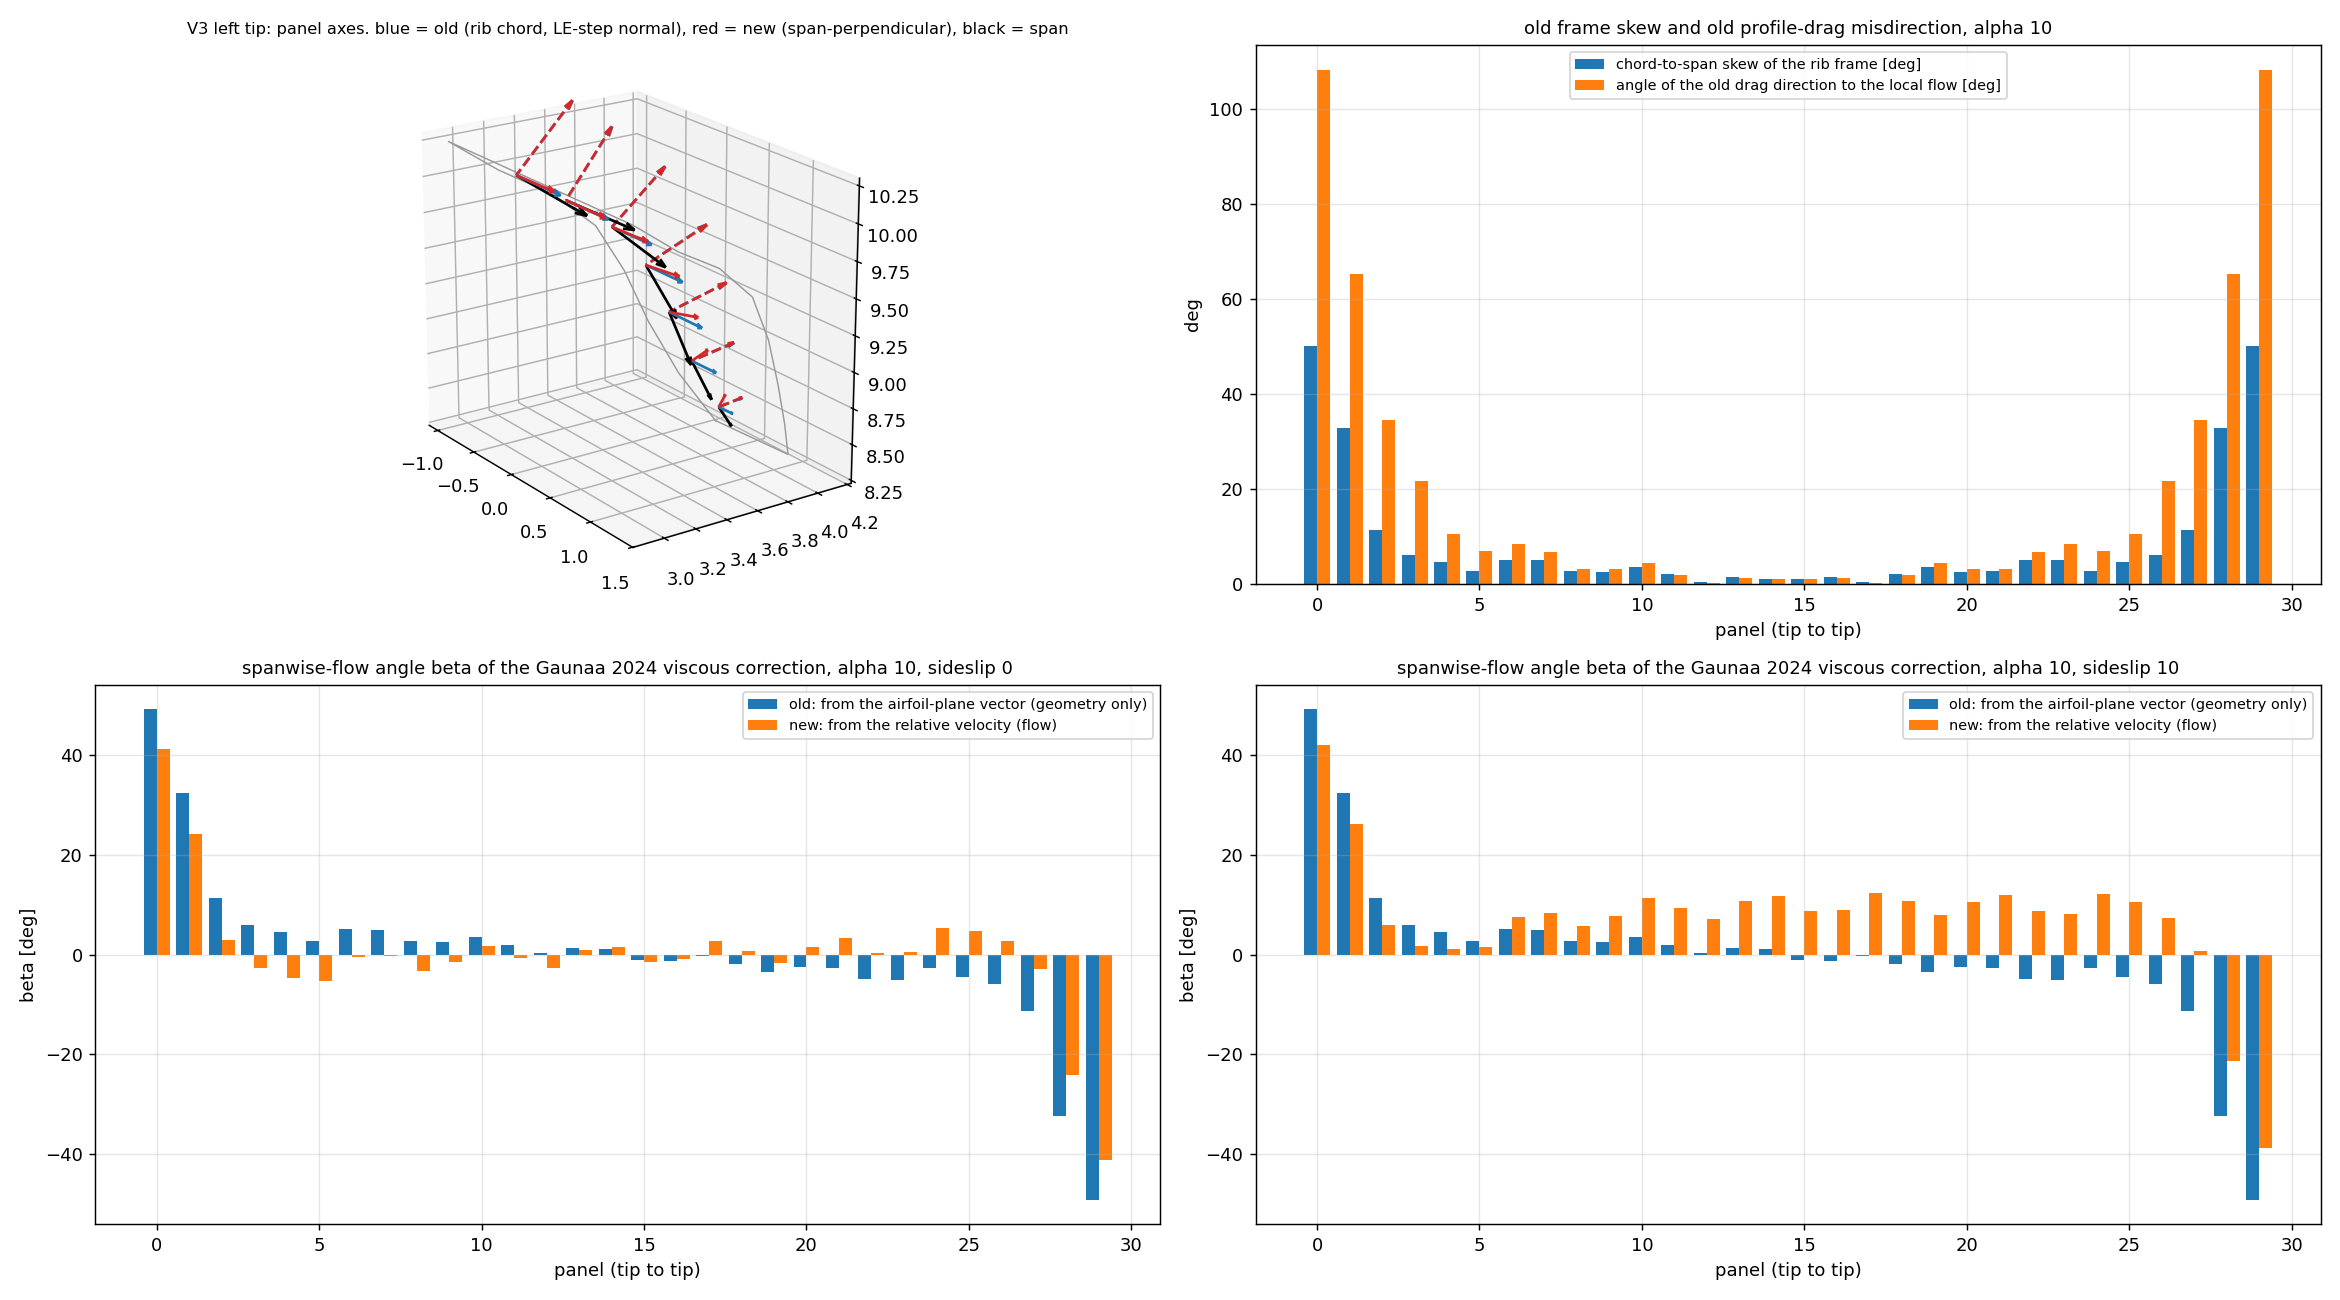
\includegraphics[width=\textwidth]{02_v3_frame_drag_direction_viscous_beta.png}
\caption{Panel frame on the V3 kite (\code{docs/figures/make\_pr\_figures.py}). Top left: the old frame built from the rib (blue) and the span-perpendicular frame of CP1 now used (red) at the left tip. Top right: the chord-to-span skew of the ribs and the angle by which a drag direction taken from the global span axis missed the local flow, up to $108^\circ$ at the tips. Bottom: the spanwise-flow angle $\beta$ of the viscous correction (Section~\ref{sec:viscous}) from the geometry alone (old) and from the relative velocity (new), at $0$ and $10^\circ$ sideslip.}
\label{fig:frame}
\end{figure}

\section{The vortex system}
\label{sec:vortex}
\paragraph{Filaments} (\code{Panel}, \code{Filament}). Each panel carries a ring of five filaments of strength $\Gamma_i$ (Figure~\ref{fig:legs}): the bound segment $\vect b_2\to\vect b_1$ on the quarter-chord line, two attached-trailed legs from the bound points to the trailing-edge points $\vect T_1$, $\vect T_2$, and two semi-infinite wake filaments from $\vect T_1$ and $\vect T_2$ along the local apparent velocity, with opposite sense. Neighbouring panels share a section boundary, so the net trailed strength on boundary $j$ is $\Gamma_j-\Gamma_{j-1}$, as Helmholtz' theorems require.

\paragraph{Induced velocities.} A straight segment $\vect A\to\vect B$ of strength $\Gamma$ induces at $\vect P$, with $\vect r_0=\vect B-\vect A$, $\vect r_1=\vect P-\vect A$, $\vect r_2=\vect P-\vect B$,
\begin{equation}
\vect u=\frac{\Gamma}{4\pi}\,\frac{\vect r_1\times\vect r_2}{|\vect r_1\times\vect r_2|^2}\;\vect r_0\cdot\Big(\frac{\vect r_1}{|\vect r_1|}-\frac{\vect r_2}{|\vect r_2|}\Big),
\label{eq:segment}
\end{equation}
and a semi-infinite filament from $\vect A$ along the unit direction $\vect e$,
\begin{equation}
\vect u=\frac{\Gamma}{4\pi}\,\frac{1+\vect r_1\cdot\vect e/|\vect r_1|}{|\vect r_1\times\vect e|^2}\;\vect r_1\times\vect e .
\label{eq:semiinf}
\end{equation}
Near a filament the velocity is regularised. The bound segments use a Vatistas core of radius $\epsilon_1=\delta\,|\vect r_0|$ with $\delta$ the \code{core\_radius\_fraction} (default $10^{-20}$, i.e.\ no core: the model never evaluates a bound segment on its own line, Section~\ref{sec:curved}); the legs and the wake use the viscous core of~\cite{damiani2019}, $\epsilon_2=\sqrt{4\alpha_0\nu\,r_\perp/U}$ with the Oseen parameter $\alpha_0=1.25643$, $\nu$ the kinematic viscosity and $r_\perp$ the distance along the filament to the foot of the evaluation point. Inside a core the velocity ramps linearly to zero; on the line it is zero.

\paragraph{Influence matrices} (\code{BodyAerodynamics.compute\_AIC\_matrices}, \code{utils.assemble\_AIC\_matrices}). The velocity induced at every evaluation point by every ring of unit strength is assembled once per inflow into three $N\times N$ matrices, $\vect u=\mathrm{AIC}_x\boldsymbol\Gamma$ etc., evaluated with a numba kernel. For the VSM the evaluation points are the control points and the bound segment of the panel's own ring is included; for the LLT variant they are the aerodynamic centres and the own bound segment is excluded (it induces nothing on its own line). In the VSM the two-dimensional velocity of an infinite vortex of the panel's own strength along its bound direction is subtracted at its control point (TAT1 of~\cite{gaunaa2026}, Section~\ref{sec:coupling}), so that the inner model sees the three-dimensional disturbance only.

\paragraph{Wake direction} (\code{Wake.frozen\_wake}). Each ring's wake follows that panel's own apparent velocity: the freestream plus the body-rate term, or the distributed inflow. In a uniform inflow this is the classical single straight wake; under yaw or roll rates it is locally aligned. On a translating wing the wake direction is a second-order effect (a per-panel wake changes the V3 lift by under 1\,\%).

\paragraph{Direction of the attached-trailed legs} (\code{leg\_direction}, Figure~\ref{fig:legs}). Theory does not fix the path of the attached vorticity between the bound vortex and the trailing edge; \cite{gaunaa2026} calls it a modelling choice and takes the chordwise direction of CP1. The code offers three constructions. \code{"rib"} (default) runs the legs along the interpolated sections to their trailing-edge points, with the control point on the section: a fixed vortex system, independent of the inflow. \code{"streamwise"} runs them along the mean apparent velocity projected onto the surface, up to the trailing-edge curve, rebuilt whenever the inflow is set. \code{"perpendicular"} is the paper's construction, with the quarter-chord tangent averaged over one leg length so that the legs fan out instead of crossing at a planform kink. In the last two the control point moves with the legs so that it stays between the panel's own two legs. Section~\ref{sec:val-legs} compares the three against a vortex-lattice method; the rib legs are the default because the code's main use is trim finding with an inflow that varies along the span, where only the rib construction is unambiguous, and their accuracy is the same.

\begin{figure}[p]\centering
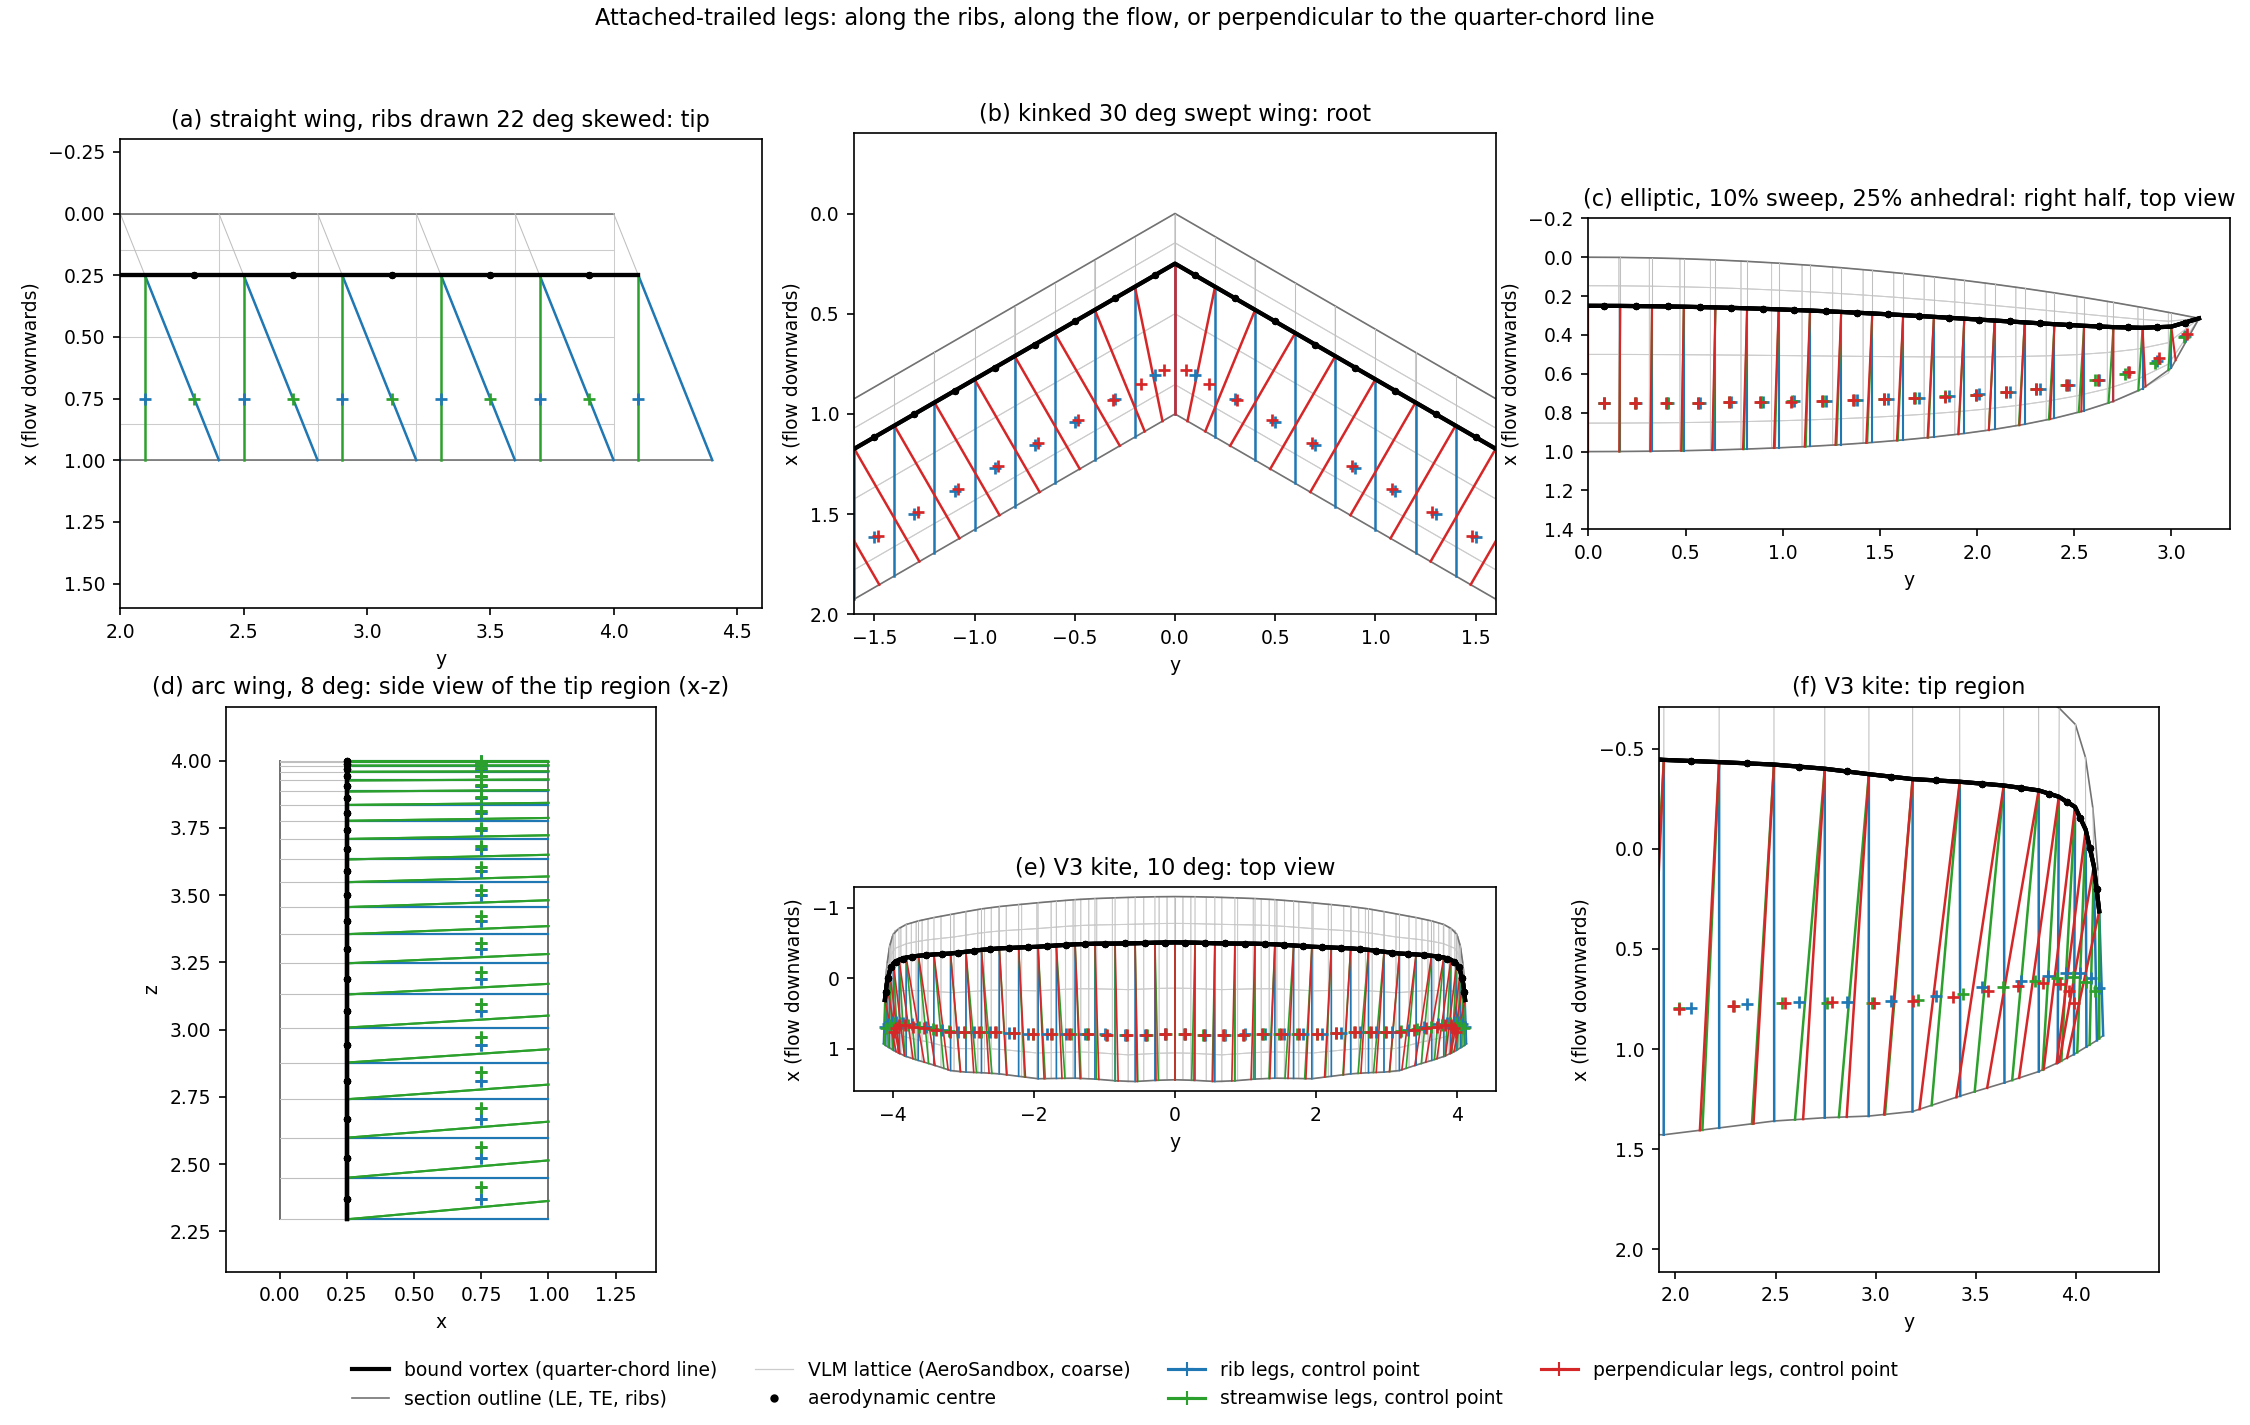
\includegraphics[width=\textwidth]{10_leg_direction_geometry.png}
\caption{The vortex system seen from above (flow downwards) and from the side for the three leg constructions (\code{docs/validation/leg\_direction\_study.py --figures}): bound vortex (black), aerodynamic centres (dots), control points (crosses in the colour of their legs), rib legs (blue), streamwise legs (green), perpendicular legs (red), and the lattice of the vortex-lattice referee of Section~\ref{sec:val-legs} in grey. (a) A straight wing whose ribs are drawn skewed; (b) the root of a kinked swept wing; (c) a swept--anhedral elliptic wing; (d) the arc wing from the side, where streamwise legs climb along the nearly vertical tips; (e, f) the V3 kite and its tip.}
\label{fig:legs}
\end{figure}

\section{The inner--outer coupling}
\label{sec:coupling}
This section follows the coupling rules of Gaunaa, Li and Pirrung~\cite{gaunaa2026}, which the code implements in full except for the direction of the legs (previous section) and the treatment of the curved bound vortex at the quarter chord (Section~\ref{sec:curved}). The rules are: CP1, only the span-perpendicular velocity drives the inner model; TAT1, that velocity excludes the section's own two-dimensional disturbance; TAT2, the magnitude of the sectional force follows from the flow at the three-quarter chord; TAT3, its direction from the flow at the quarter chord.

\subsection{Inner velocity and circulation}
\label{sec:gamma}
At the control point $\vect C_i$ the three-dimensional relative velocity is the apparent velocity plus the induced velocity of the whole vortex system, $\vect V_{3D,i}=\vect V_{a,i}+\sum_j \mathrm{AIC}_{ij}\Gamma_j$. The inner velocity is its span-perpendicular part minus the two-dimensional disturbance of the section's own bound vortex (CP1 and TAT1):
\begin{equation}
\vect V_{\mathrm{inner},i}=\vect V_{3D,i}-(\vect V_{3D,i}\cdot\vect e_{s,i})\vect e_{s,i}-\vect V_{2D,\mathrm{bound},i},\qquad
\alpha_{3/4,i}=\operatorname{atan2}(\vect V_{\mathrm{inner},i}\cdot\vect e_{n,i},\ \vect V_{\mathrm{inner},i}\cdot\vect e_{c,i}),
\end{equation}
and the circulation follows from the sectional lift (eq.~4 of~\cite{gaunaa2026}, TAT2):
\begin{equation}
\Gamma_i=\tfrac12\,|\vect V_{\mathrm{inner},i}|\,c_i\,C_{l,i}(\alpha_{3/4,i}).
\label{eq:gamma}
\end{equation}
For a flat plate, $C_l=2\pi\alpha$, this is Weissinger's three-quarter-chord condition: on an infinite wing the bound vortex at $c/4$ induces at $3c/4$ exactly the downwash that makes the flow tangent there. On a swept infinite wing the perpendicular chord and velocity in~\eqref{eq:gamma} give the lift slope $2\pi\cos\Lambda$ of simple sweep theory; a streamwise chord would not.

\subsection{Force magnitudes and directions}
\label{sec:forces}
The sectional lift, drag and moment per unit span use the inner velocity and the polar at $\alpha_{3/4}$:
\begin{equation}
L'_i=\tfrac12\rho|\vect V_{\mathrm{inner},i}|^2 c_i C_{l,i},\qquad D'_i=\tfrac12\rho|\vect V_{\mathrm{inner},i}|^2 c_i C_{d,i},\qquad M'_i=\tfrac12\rho|\vect V_{\mathrm{inner},i}|^2 c_i^2 C_{m,i},
\end{equation}
multiplied by the panel width along the bound vortex. Their directions follow TAT3: the lift is perpendicular and the drag parallel to the undisturbed relative flow at the quarter chord, $\vect V_{1/4,i}$, within the span-normal plane (\code{is\_aoa\_corrected=True}, the default). $\vect V_{1/4,i}$ is the apparent velocity plus the induction of the trailed system (legs and wake of every ring) at $\vect P_i$, which for a straight wing is Prandtl's exact downwash, plus the influence of the curved or swept bound vortex of the next section. Taking the directions from the three-quarter-chord flow instead (\code{is\_aoa\_corrected=False}, the paper's LL-3/4) overestimates the induced drag by 20--40\,\%, Section~\ref{sec:val-trefftz}. The moment acts about the bound vortex, with the polar's $C_m$ referred to the quarter chord.

\subsection{The curved bound vortex at the quarter chord}
\label{sec:curved}
On a curved or swept quarter-chord line the neighbouring bound segments induce a velocity at $\vect P_i$ that grows as the logarithm of the panel width: the lifting line evaluated on itself is singular (Li et al.~\cite{li2020}). The on-blade induced drag is $\rho\Gamma(w\cos\alpha+u\sin\alpha)$ with $w$ an induced angle of about one degree, so a chordwise velocity $u$ of 3\,\% of the freestream moves the drag by 12\,\%; evaluating the other panels' segments on the line made the V3 induced drag fall from 0.93 to 0.86 of the Trefftz value between 20 and 150 panels. The code regularises the term without a free parameter~\cite{report}: for each panel $i$ the wing is unrolled onto the tangent line of panel $i$, and the quarter-chord velocity is the classical downwash of the unrolled wing plus the difference between the actual and the unrolled vortex systems, both with the bound vorticity and the leg starting points spread along the chord with the thin-airfoil distribution $\gamma(x)\propto\sqrt{(c-x)/x}$ (24 strips, effective cut-off $0.15\,c$):
\begin{equation}
\vect V_{1/4,i}=\vect V_{a,i}+\sum_j\Gamma_j\Big[\vect K^{\mathrm{LL}}_{j,\mathrm{unrolled}(i)}(\vect P_i)+\vect K^{\mathrm{sheet}}_{j}(\vect P_i)-\vect K^{\mathrm{sheet}}_{j,\mathrm{unrolled}(i)}(\vect P_i)\Big].
\label{eq:curved}
\end{equation}
The bracket is identically zero on a straight wing, finite everywhere, and the wake terms cancel between the two systems. Figure~\ref{fig:unroll} shows the unrolled reference wing for two panels of an arc wing and one of a kinked swept wing: it is a different straight wing for every panel, tangent at that panel, and it coincides with the real wing in the panel's neighbourhood, which is why the singular near field cancels in the difference and only the far-field effect of the curvature remains. Implementation: \code{utils.assemble\_curved\_bound\_correction\_AIC}, about 0.5\,s at 50 panels. The matrix depends on the panel geometry only, so it is computed once per shape and reused for every inflow and circulation; a body that is the cached shape up to a rigid rotation and translation reuses the stored matrix rotated, which keeps a trim that rotates the kite for every residual evaluation at the cost of one evaluation per deformed shape. It shares its mechanism with the effective-lifting-line method of Reid and Hunsaker~\cite{reid2020}, whose two empirical lengths it replaces with the thin-airfoil distribution. Figure~\ref{fig:curved} shows the problem and the result; the full derivation, the literature and the rejected alternatives are in~\cite{report}.

\begin{figure}[p]\centering
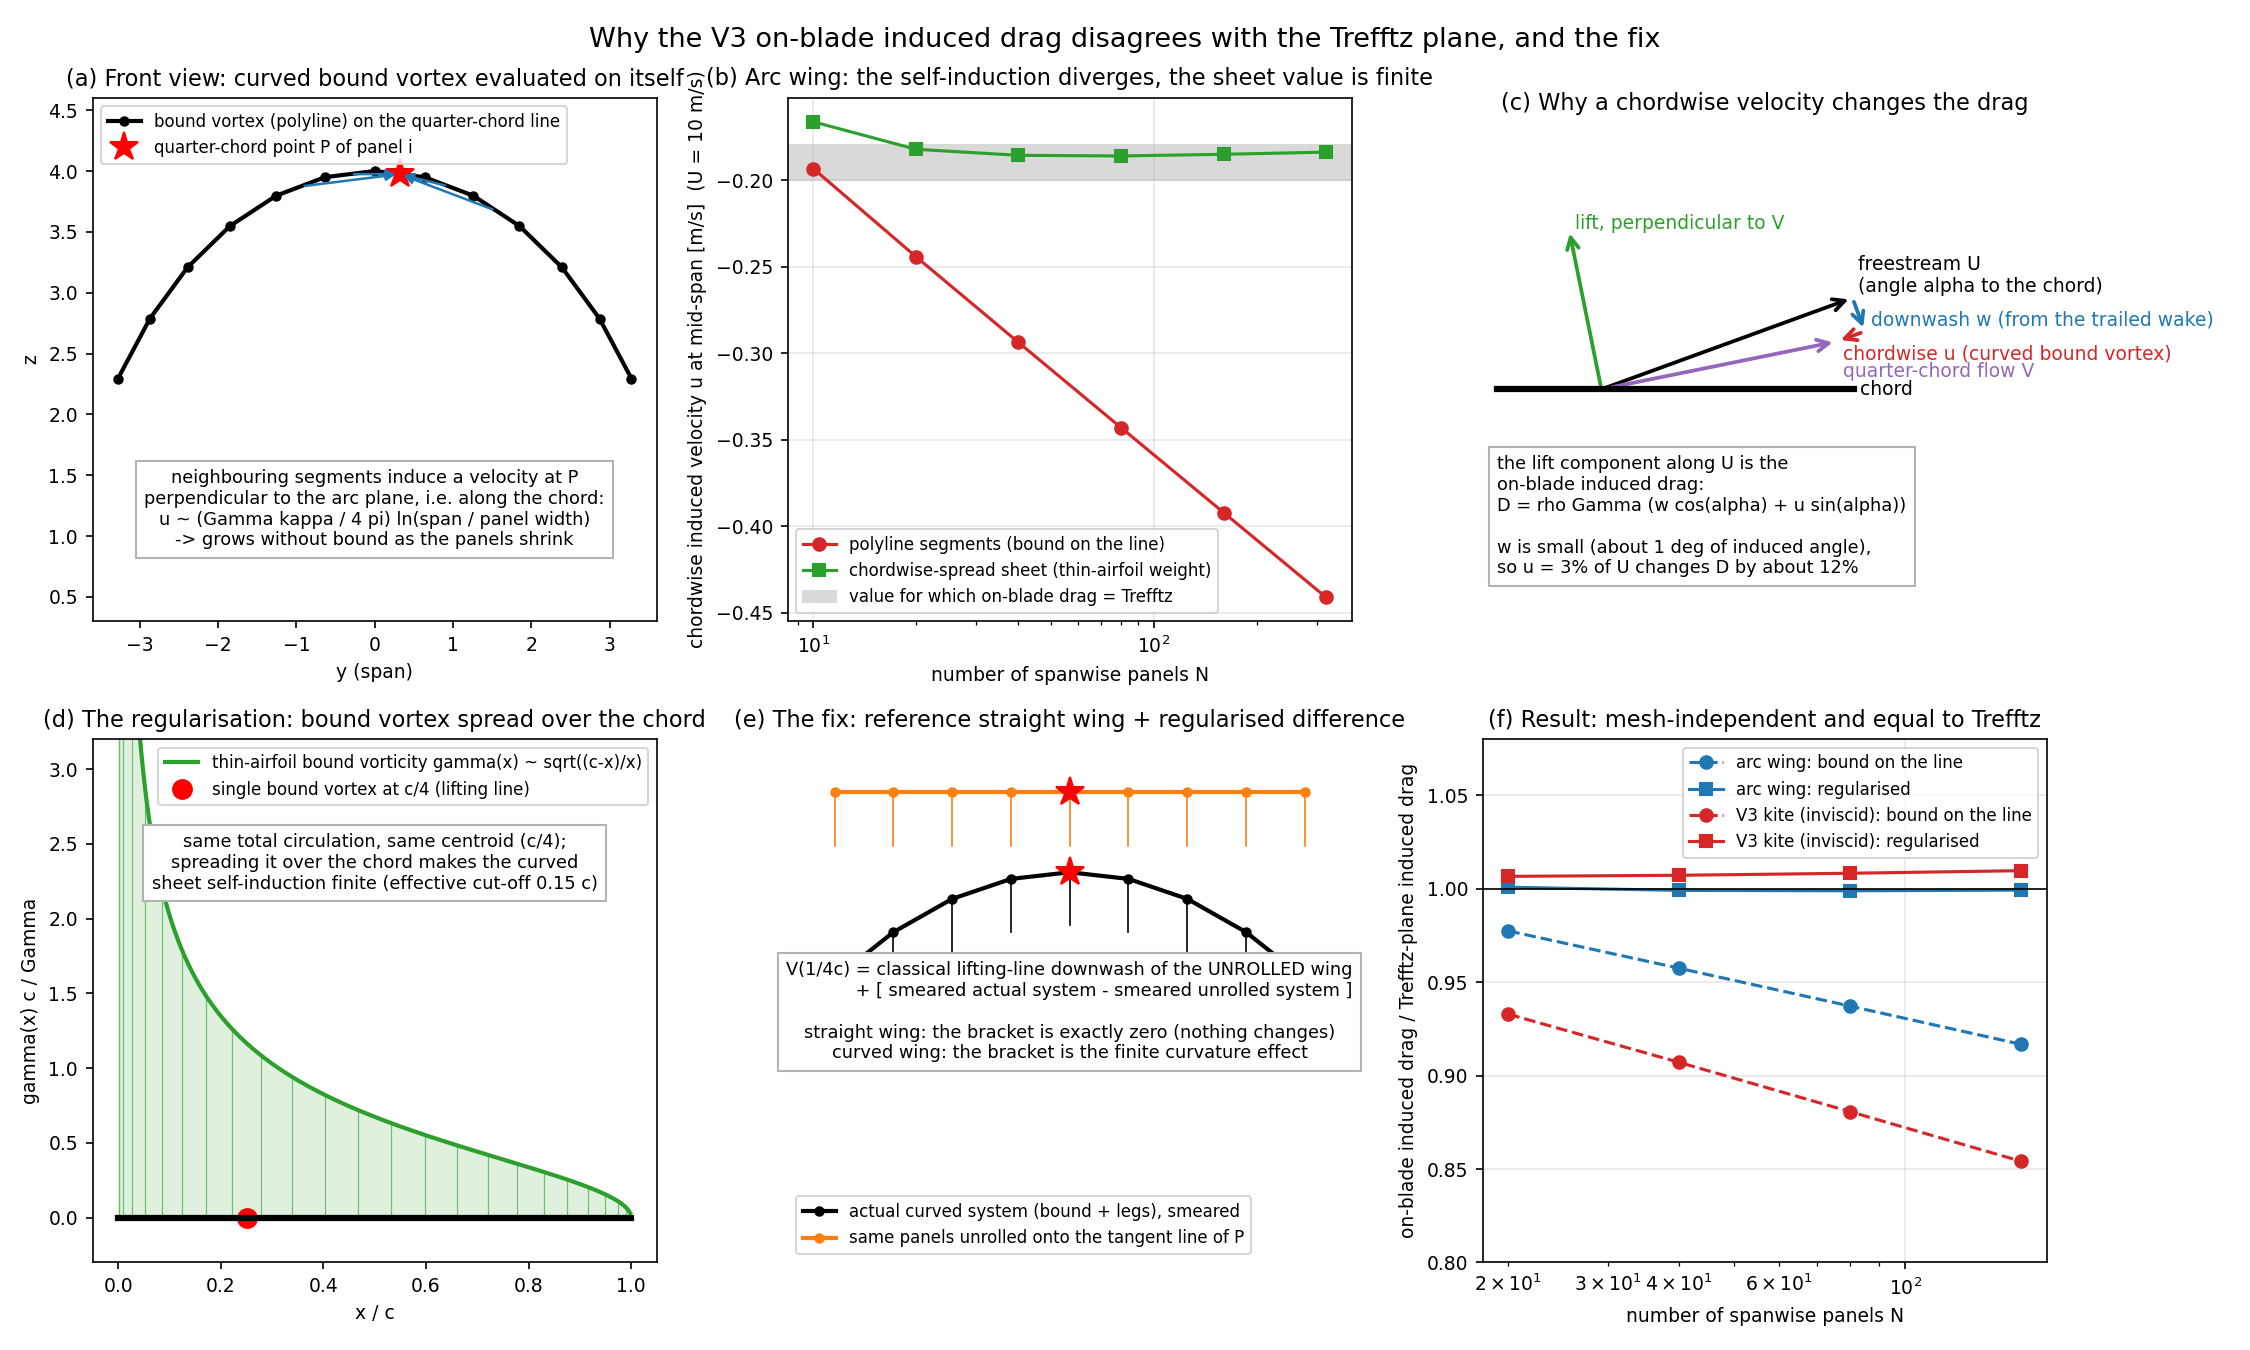
\includegraphics[width=\textwidth]{08_curved_bound_vortex_regularisation.png}
\caption{The curved bound vortex at the quarter chord (\code{docs/validation/curved\_bound\_vortex\_validation.py --figures}). (a) The log-singular self-induction of a curved line; (b) the chordwise velocity at mid-span of an arc wing from the polyline (grows with the panel count) and from the chordwise-spread sheet (finite); (c) why the drag is sensitive to it; (d) the thin-airfoil distribution; (e) the construction of eq.~\eqref{eq:curved}; (f) on-blade over Trefftz induced drag against panel count on the arc and the V3, before (dashed) and after (solid).}
\label{fig:curved}
\end{figure}

\begin{figure}[p]\centering
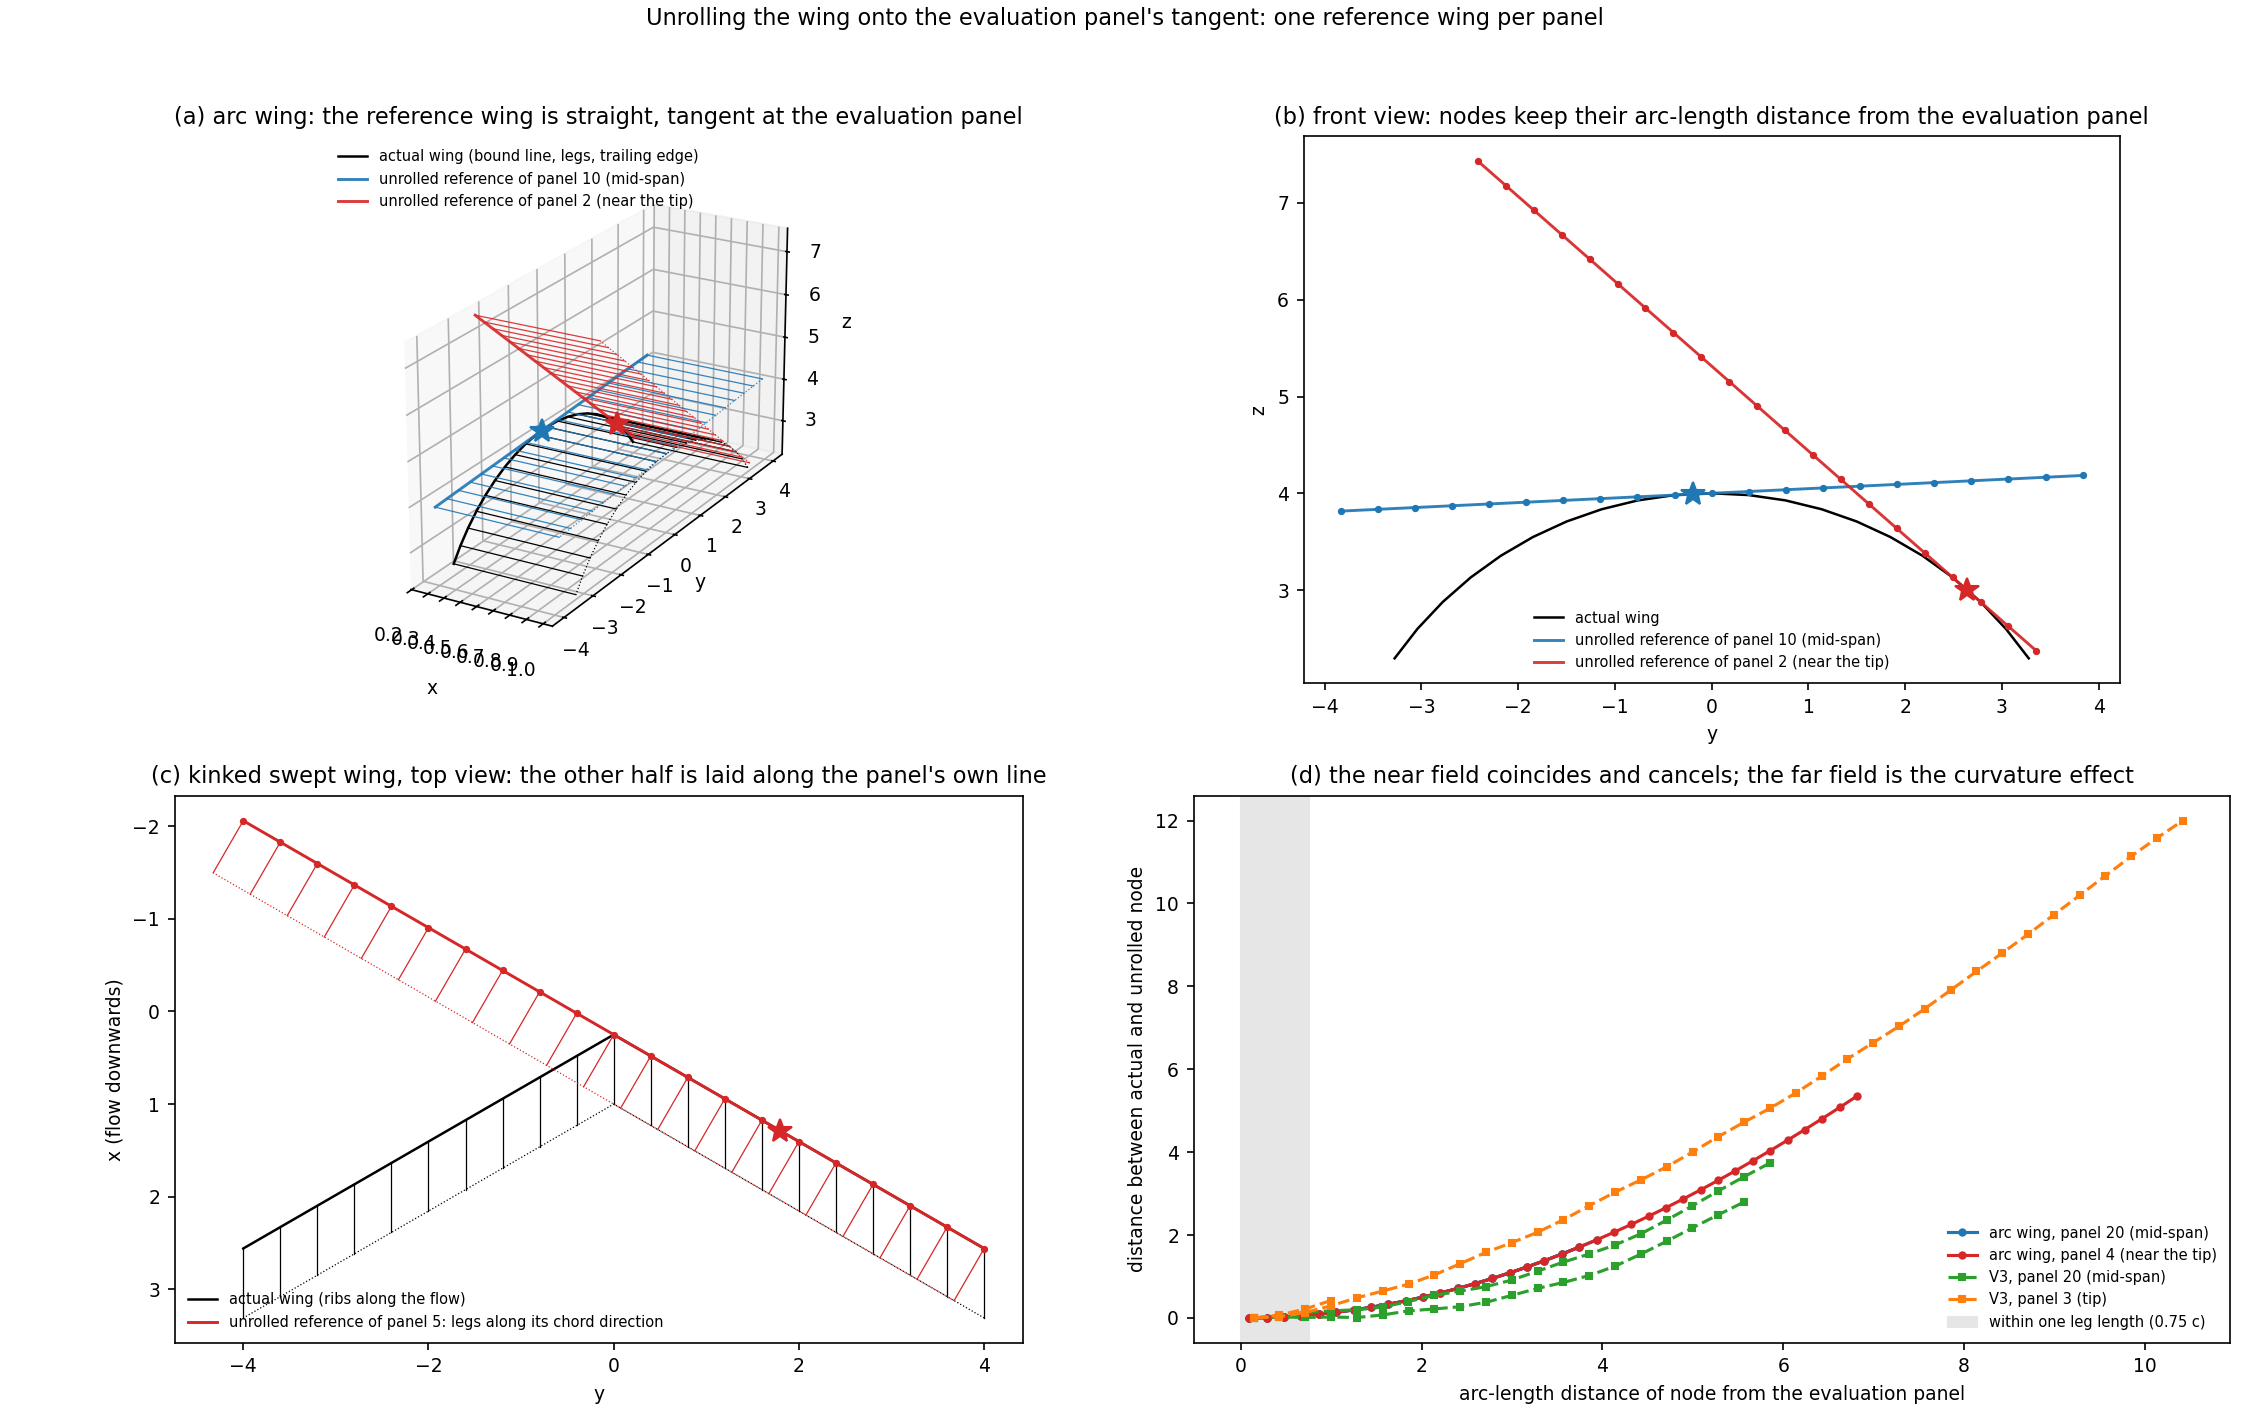
\includegraphics[width=\textwidth]{14_unrolling_per_panel.png}
\caption{Unrolling the wing onto the evaluation panel's tangent (\code{docs/validation/unrolling\_figure.py}). (a, b) Arc wing: the reference wings of a mid-span panel (blue) and a near-tip panel (red), each straight and tangent at its own panel (star), nodes at their arc-length distances. (c) Kinked swept wing from above: the reference of a panel on the right half lays the other half along that panel's line, legs along that panel's chord direction. (d) Distance between actual and unrolled nodes against their distance from the evaluation panel: the near field coincides and cancels, the far field is the curvature effect.}
\label{fig:unroll}
\end{figure}

\subsection{The attached-trailed force}
\label{sec:atforce}
The chordwise legs between the bound vortex and the trailing edge are attached to the wing and carry a Kutta--Joukowski force (Section~3 of~\cite{gaunaa2026}). On section boundary $j$, with net strength $\Delta\Gamma_j=\Gamma_j-\Gamma_{j-1}$ and leg vector $\vect l_j$,
\begin{equation}
\vect F_{\mathrm{AT},j}=\rho\,\Delta\Gamma_j\,\vect V_{3D}(\vect Q_j)\times\vect l_j,
\end{equation}
where $\vect V_{3D}(\vect Q_j)$ is the full relative velocity at the leg's three-quarter point, the point where the flow has no component through the wing. The force is spanwise and cancels on an unswept wing; on swept wings and on the curved outboard parts of a kite it changes lift and induced drag (Figure~\ref{fig:at}). It is on by default (\code{is\_with\_attached\_trailed\_vortex\_force}) and reported per boundary in \code{F\_attached\_trailed\_distribution}.

\begin{figure}[t]\centering
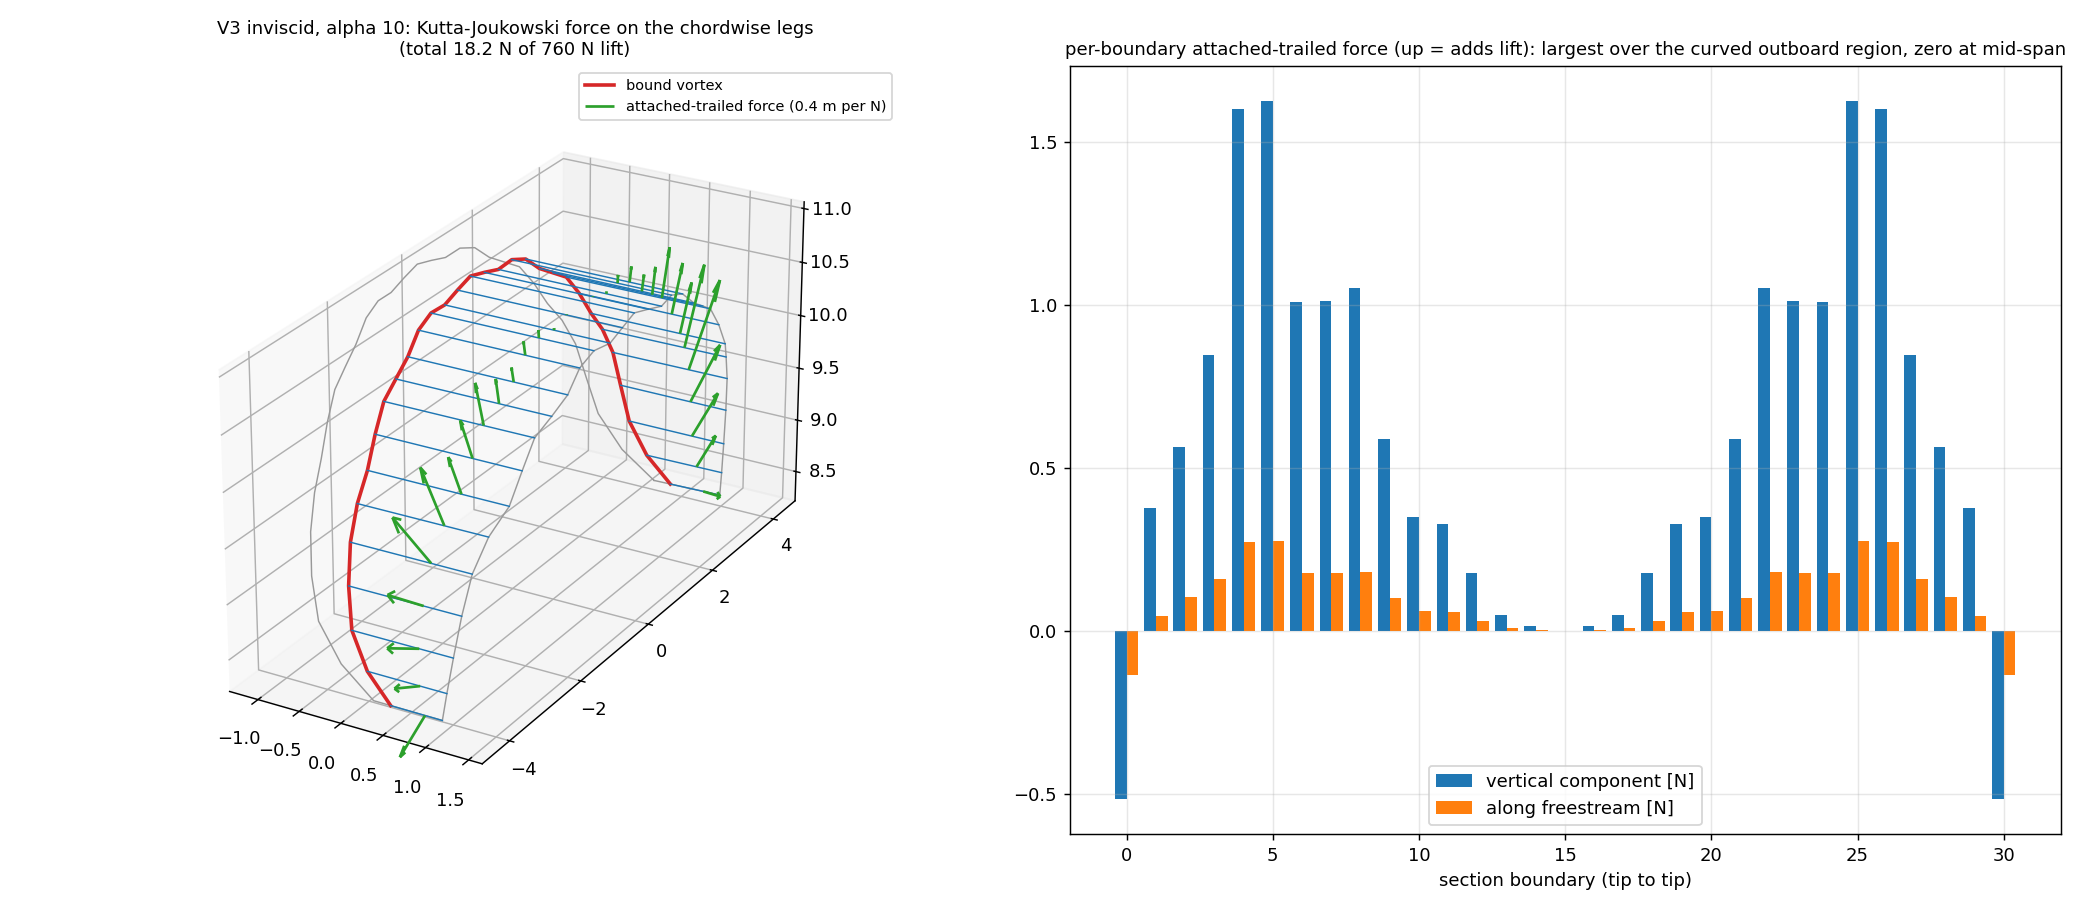
\includegraphics[width=0.9\textwidth]{04_v3_attached_trailed_force.png}
\caption{Attached-trailed force on the inviscid V3 at $10^\circ$ (\code{make\_pr\_figures.py}). Left: force vectors per section boundary. Right: vertical and streamwise components, largest over the curved outboard region and zero at mid-span where the legs follow the flow. Total 18\,N of 760\,N lift.}
\label{fig:at}
\end{figure}

\subsection{Spanwise-flow viscous correction}
\label{sec:viscous}
With \code{is\_with\_viscous\_drag\_correction} the friction force of each section is corrected for the spanwise flow following Gaunaa, Sørensen and Li~\cite{gaunaa2024}, eqs.~4, 10 and 11: with $\beta=\operatorname{atan2}(\vect V\cdot\vect e_s,\ |\vect V-(\vect V\cdot\vect e_s)\vect e_s|)$ the angle between the full relative velocity at the control point and the span-normal plane, and the Reynolds number and dynamic pressure referred to the span-normal velocity, the correction adds a drag increment along the inner flow direction and a spanwise friction force along $\vect e_s$. On the V3 it is below $0.002$ in $C_D$ even at $20^\circ$ sideslip; it is off by default.

\subsection{Stall: artificial viscosity}
\label{sec:stall}
Past the stall onset the lift slope of a polar is negative and the fixed-point iteration of Section~\ref{sec:solver} loses stability. With \code{is\_with\_artificial\_viscosity} the spanwise artificial viscosity of Li, Gaunaa, Pirrung and Lønbæk~\cite{li2026} is applied implicitly to the circulation update once any panel is past its positive or negative stall onset, with the coefficient of their eq.~16 written for a non-uniform grid and the factor $k=0.035$; it is a no-op in attached flow. It is off by default; for post-stall solutions the \code{casadi\_newton} loop is the robust alternative.

\subsection{The lifting-line variant}
\label{sec:llt}
With \code{aerodynamic\_model\_type="LLT"} the inner velocity is evaluated at the aerodynamic centre and the own bound segment is excluded; no two-dimensional subtraction and no quarter-chord correction are needed. This is Prandtl's lifting line with nonlinear polars, exact for straight wings of high aspect ratio and provided for comparison; the VSM is the model for curved, swept and low-aspect-ratio wings.

\section{Solver, inflow and outputs}
\label{sec:solver}
\paragraph{Iteration} (\code{Solver.solve}). With the influence matrices assembled, the circulation is the fixed point of~\eqref{eq:gamma}. The base loop is an under-relaxed fixed-point iteration, $\boldsymbol\Gamma\leftarrow(1-\omega)\boldsymbol\Gamma+\omega\,\boldsymbol\Gamma_{\mathrm{new}}(\boldsymbol\Gamma)$, stopped when $\max|\Delta\Gamma|/\max|\Gamma|<$ \code{allowed\_error} ($10^{-6}$). The relaxation factor defaults to $0.8$ times the stability limit of~\cite{li2026}, eq.~11, evaluated on the actual panels and polars,
\begin{equation}
\omega_{\max}=\frac{2}{1+\tfrac14\max_i (c_i/\Delta s_i)\,C_{l,i}'},
\end{equation}
exact for the LLT and halved for the VSM, whose three-quarter-chord control point sees about twice the trailed induction (measured 0.51--0.66, Figure~\ref{fig:relax}). Alternatives: Anderson acceleration (10--25 times fewer iterations in attached flow), a Newton loop with an exact CasADi Jacobian and pseudo-transient continuation (3--10 iterations, converges post-stall), and Broyden solvers. The initial circulation is elliptic, cosine, zero or a previous solution.

\begin{figure}[t]\centering
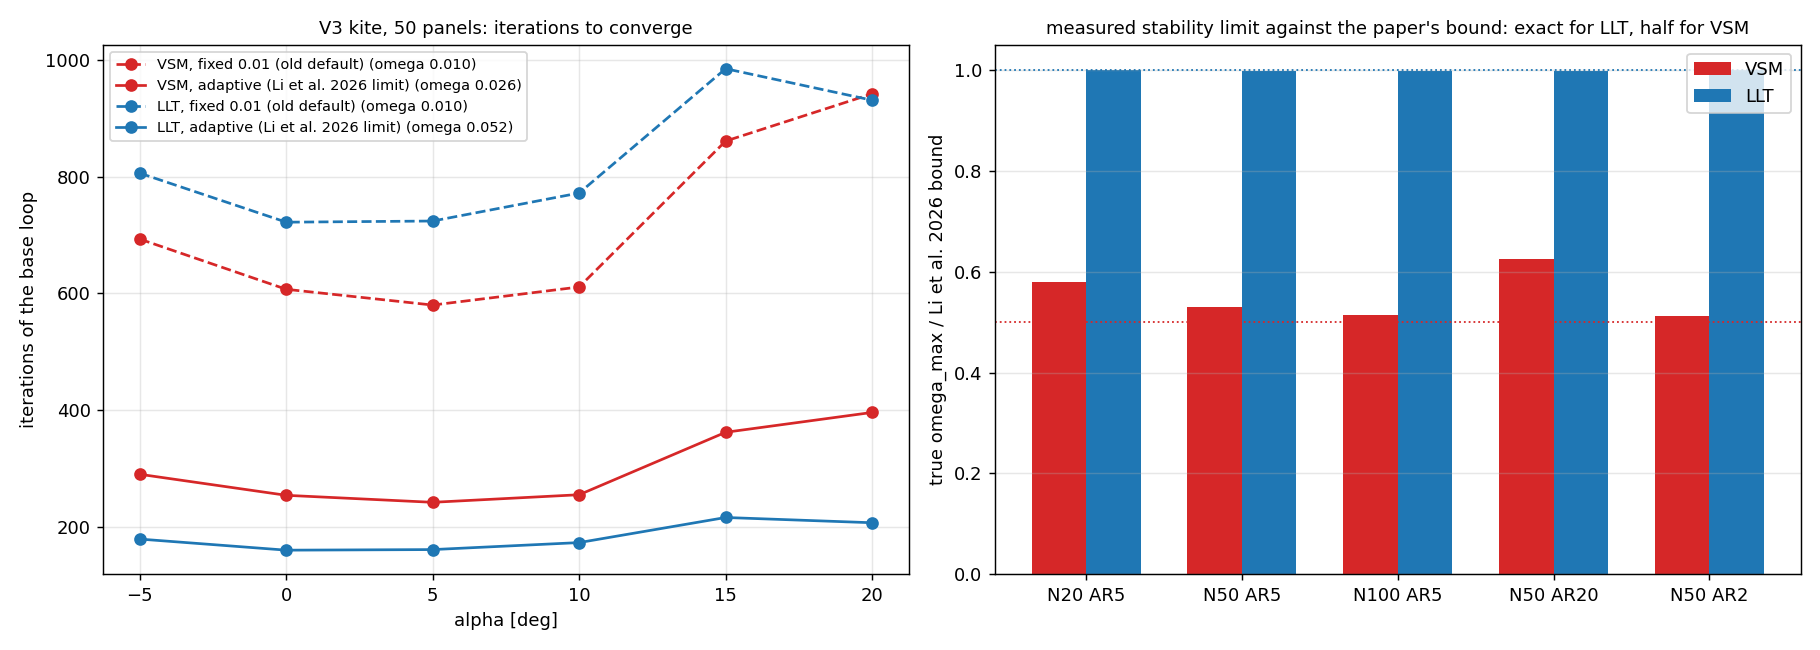
\includegraphics[width=0.9\textwidth]{05_relaxation_factor.png}
\caption{Relaxation factor (\code{make\_pr\_figures.py}). Left: iterations on the V3 with the old fixed $0.01$ and with the default derived from the stability limit, for VSM and LLT. Right: the measured stability limit over the bound of~\cite{li2026} on rectangular wings: exact for the LLT, about half for the VSM.}
\label{fig:relax}
\end{figure}

\paragraph{Inflow} (\code{BodyAerodynamics.va}, \code{va\_initialize}). The apparent velocity is a single vector (speed, angle of attack, sideslip), or one vector per panel, optionally with rigid-body rates about given axes through a reference point: $\vect V_{a,i}=\vect V_\infty-\boldsymbol\omega\times(\vect C_i-\vect r_0)$. The sign conventions are in Section~\ref{sec:conventions}. Each inflow rebuilds the wake (and, with streamwise legs, the legs).

\paragraph{Forces, moments and coefficients} (\code{BodyAerodynamics.compute\_results}). Panel forces are summed in the global frame; lift, drag and side force are the components along the reference wind axes, built from a reference velocity $\vect V_{\mathrm{ref}}$ (the panel inflow when it is uniform, otherwise an area-weighted root-mean-square of the distribution without the rotational term) and the span direction: drag along $\vect V_{\mathrm{ref}}$, lift along $\vect V_{\mathrm{ref}}\times\vect e_{\mathrm{span}}$, side force completing the triad. Coefficients use $q_{\mathrm{ref}}=\tfrac12\rho|\vect V_{\mathrm{ref}}|^2$ and the projected area $S$ of the wing onto the $z$-plane; moment coefficients are further divided by the largest chord. The results dictionary also carries the spanwise distributions of $\Gamma$, $\alpha$, the sectional coefficients, the panel forces and moments, the centre of pressure, the Reynolds number on the largest chord, and the Trefftz-plane induced drag.

\paragraph{Trefftz-plane induced drag} (\code{compute\_trefftz\_plane\_induced\_drag}, reported as \code{drag\_induced\_trefftz}). For a wing in one uniform inflow the far-wake induced drag of the converged circulation is computed in the plane perpendicular to the freestream from the trace of the frozen wake: each section boundary sheds a line vortex of strength $\Delta\Gamma_j$, and $D_i=\tfrac12\rho\sum_j\Gamma_j w_{n,j}\Delta s_j$ with $w_n$ the normal induced velocity on the trace. It depends only on the circulation and the wake, not on where the forces are evaluated on the blade, and is the referee of Section~\ref{sec:val-trefftz}. It is \code{None} with body rates or a distributed inflow.

\paragraph{Bridle lines} (\code{compute\_line\_aerodynamic\_force}). Each line is a cylinder of length $\ell$ and diameter $d$ at angle $\theta$ to the local flow, with the cross-flow drag coefficient $C_{d,c}=1.1$ and the friction coefficient $C_f=0.01$: $C_{d,t}=C_{d,c}\sin^3\theta+\pi C_f\cos^3\theta$ along the flow and $C_{l,t}=C_{d,c}\sin^2\theta\cos\theta-\pi C_f\sin\theta\cos^2\theta$ normal to it, on the area $\ell d$. On the V3 the bridles add a constant $0.036$--$0.040$ to $C_D$; they matter for flight, not for the wind-tunnel model, which had none.

\section{Validation}
\label{sec:validation}
The validation is layered: analytical results for what theory fixes exactly, an internal consistency check for the induced drag, an independent potential-flow referee (a vortex-lattice method) for lift and induced drag on wings where no analytical result exists, and RANS and wind-tunnel data for the real kite. Inviscid polars ($C_l=2\pi\alpha$, $C_d=0$) are used wherever the comparison is with potential-flow theory, so that the lifting line and the referee solve the same problem.

\subsection{Analytical cases}
\label{sec:val-analytical}
\paragraph{Horseshoe vortices.} The induced velocity of three horseshoe vortices of prescribed strengths at a prescribed point is compared with the hand-computed Biot--Savart result (the \code{analytical\_horshoe\_vortices} case in \code{tests/verification\_cases}); it checks eqs.~\eqref{eq:segment} and~\eqref{eq:semiinf} and the sign conventions of the ring.

\paragraph{Elliptic wings.} For an elliptic planform Prandtl's lifting line gives $C_L=2\pi\alpha/(1+2/\mathrm{AR})$ and $C_{D_i}=C_L^2/(\pi\mathrm{AR})$. Figure~\ref{fig:classical} compares the LLT and the VSM with these on wings of aspect ratio 20 and 4 with a straight quarter-chord line (cosine spacing, 60 panels), and with the vortex-lattice method of Section~\ref{sec:val-legs}; the numbers are in Table~\ref{tab:classical}. The LLT reproduces the theory it discretises: lift slope within $0.4$ and $1.4\,\%$, Oswald factor $0.997$ at both aspect ratios. The VSM, which does not assume a high aspect ratio, matches the theory at aspect ratio 20 (slope $-1.5\,\%$, Oswald $0.991$) and at aspect ratio 4 follows the lifting-surface solution instead of the line theory: its lift is within $1\,\%$ of the VLM at $4$, $8$ and $12^\circ$, where Prandtl's result is $11$--$12\,\%$ too high, with the Oswald factor $0.998$. The same elliptic planform drawn with a straight leading edge has a curved quarter-chord line; the LLT variant has no regularisation for that (Section~\ref{sec:curved}) and its on-blade induced drag then exceeds its own Trefftz value by $11\,\%$ at aspect ratio 20 and $36\,\%$ at aspect ratio 4, while the VSM stays within $2\,\%$. The regression test \code{tests/verification\_cases/elliptical\_wing} holds the LLT within $0.01$ in $C_L$ and $0.001$ in $C_{D_i}$ of the theory.

\begin{figure}[t]\centering
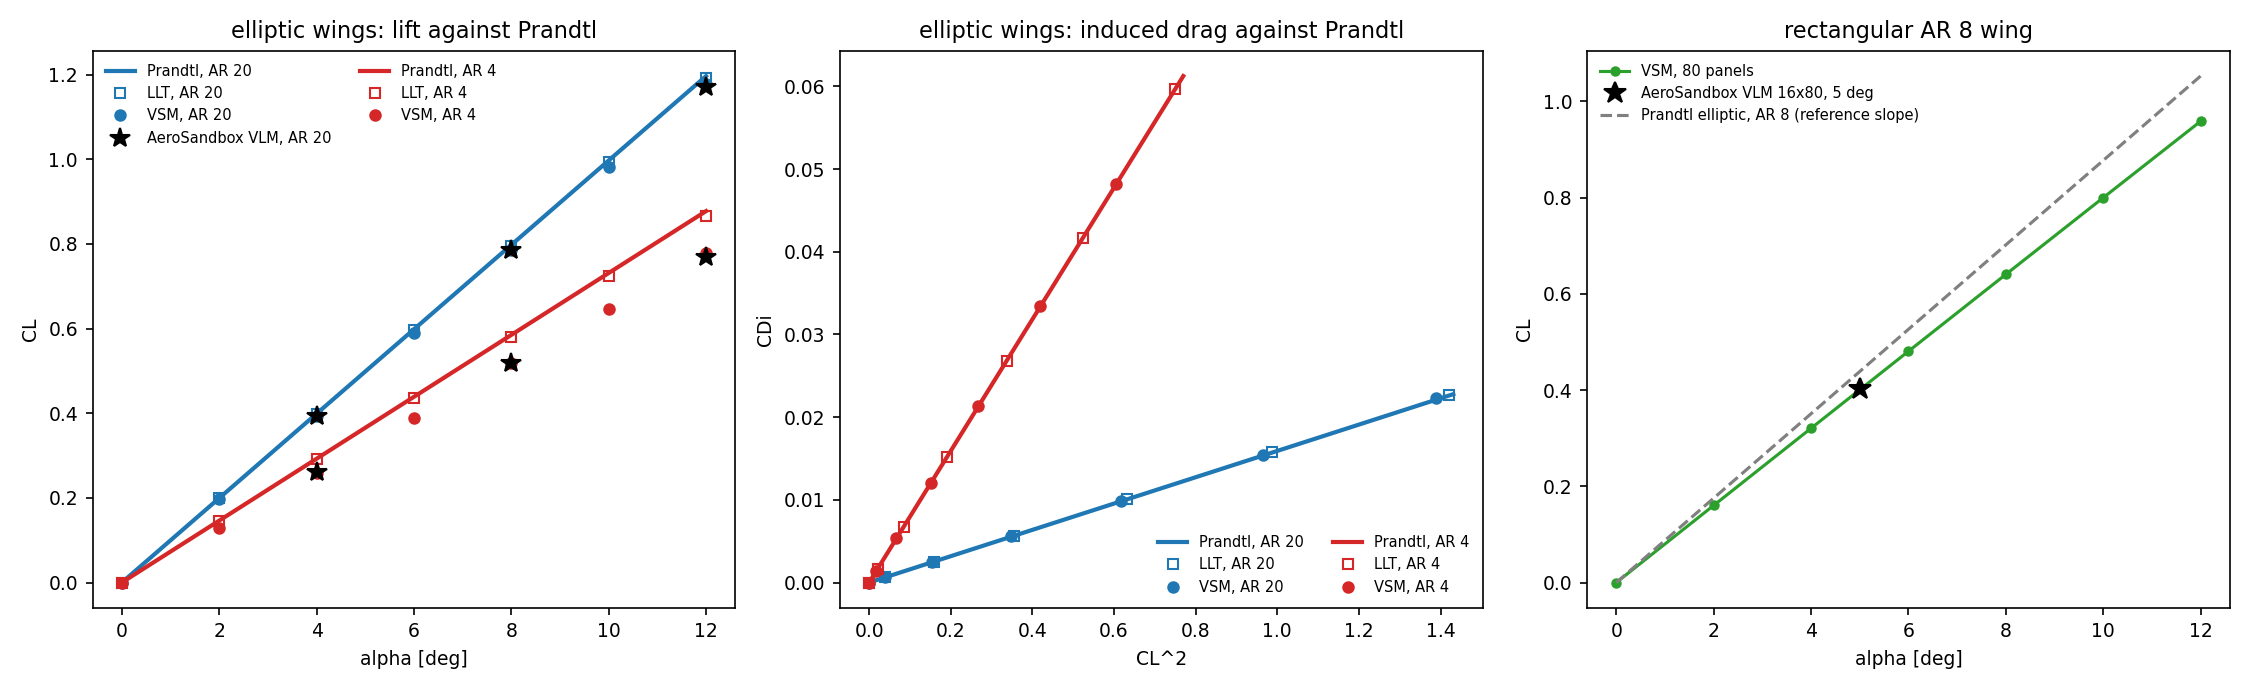
\includegraphics[width=\textwidth]{12_classical_wings.png}
\caption{Classical wings (\code{docs/validation/aerodynamic\_model\_figures.py}). Left and middle: elliptic wings of aspect ratio 20 and 4, LLT and VSM against Prandtl's lifting line and the AeroSandbox vortex-lattice method (stars). Right: the rectangular AR 8 wing, VSM against the VLM at $5^\circ$ and the elliptic reference slope.}
\label{fig:classical}
\end{figure}

\begin{table}[t]\centering\small
\caption{Classical wings: lift slope relative to Prandtl's $2\pi/(1+2/\mathrm{AR})$ and Oswald factor (inviscid polars, 60 panels, cosine spacing, straight quarter-chord line); rectangular AR 8 wing relative to the vortex-lattice method (80 panels, $5^\circ$, Table~\ref{tab:referee}).}
\label{tab:classical}
\begin{tabular}{lcc}
\toprule
case & lift slope / theory & Oswald factor\\
\midrule
elliptic AR 20, LLT & 0.996 & 0.997\\
elliptic AR 20, VSM & 0.985 & 0.991\\
elliptic AR 4, LLT & 0.987 & 0.997\\
elliptic AR 4, VSM & 0.886 & 0.998\\
\midrule
 & $C_L$ / VLM & $C_{D_i}$ / VLM\\
rectangular AR 8, VSM & 0.998 & 0.991\\
\bottomrule
\end{tabular}
\end{table}

\subsection{Consistency of the induced drag: the Trefftz plane}
\label{sec:val-trefftz}
For a given circulation and frozen wake the Trefftz-plane drag is the far-field value; a force model that evaluates the forces on the blade with the correct local flow must reproduce it, independently of the panel count. Figure~\ref{fig:trefftz} shows the on-blade over Trefftz ratio on inviscid wings. With quarter-chord directions, the attached-trailed force and the curved bound-vortex regularisation it is $1.000$ on straight wings, within $2\,\%$ on the elliptic swept--anhedral wing and the $30^\circ$ swept wing, and within $2\,\%$ on the V3 at $5$, $10$ and $15^\circ$, at every resolution. Three-quarter-chord directions overshoot by 20--40\,\%. Before the regularisation the V3 ratio fell with the panel count (0.93, 0.90, 0.86 at 20, 50, 150 panels). The check is a consistency test of the force evaluation, not a validation of the circulation; that is what the next subsection does.

\begin{figure}[t]\centering
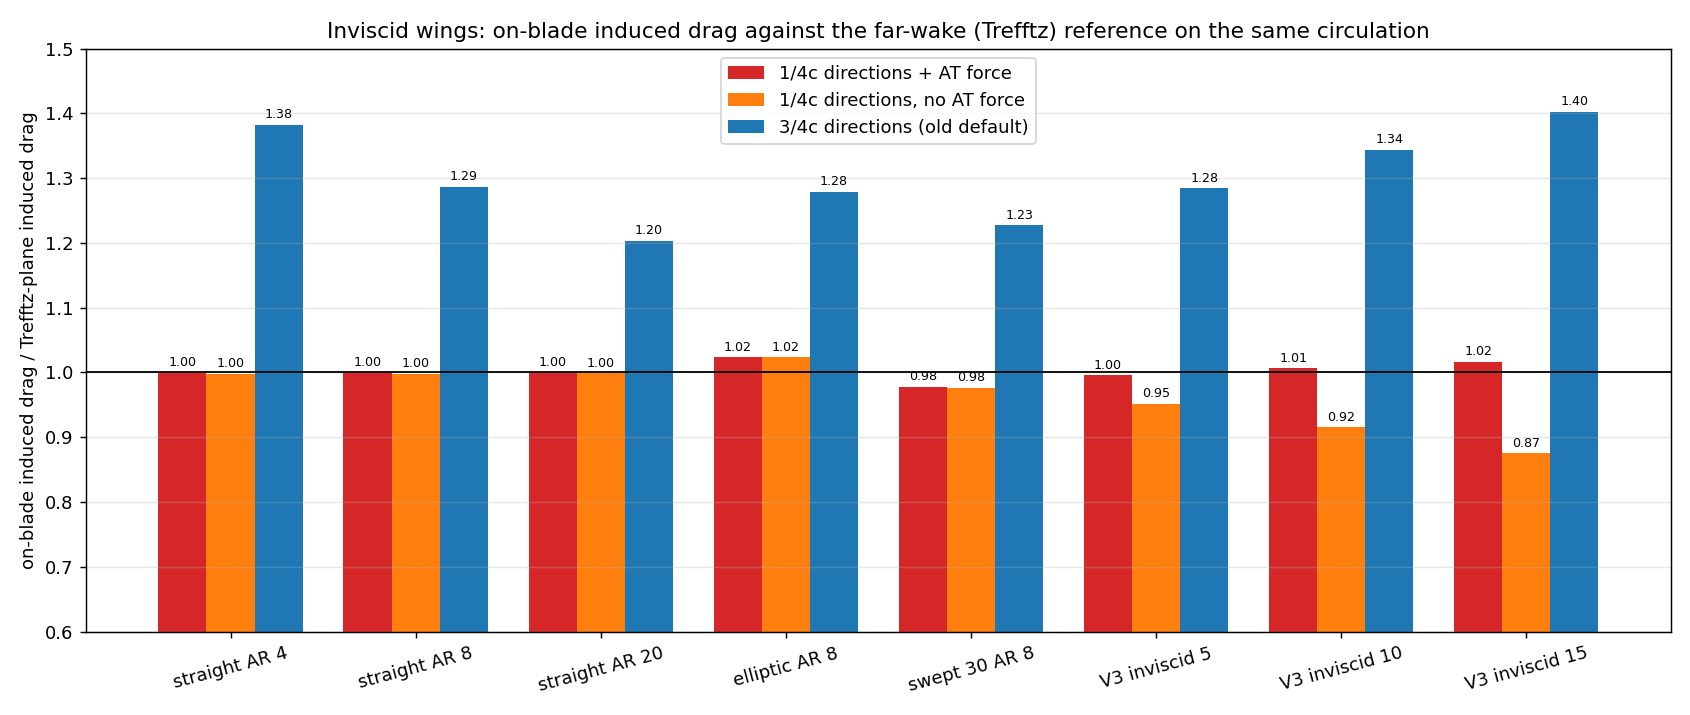
\includegraphics[width=\textwidth]{03_trefftz_check.png}
\caption{On-blade over Trefftz-plane induced drag on inviscid wings against panel count (\code{make\_pr\_figures.py}); the ratio must be one for a consistent force model.}
\label{fig:trefftz}
\end{figure}

\subsection{Vortex-lattice referee: lift and induced drag on planar, swept, curved and kite-like wings}
\label{sec:val-legs}
The Trefftz plane cannot judge the lift. For that the vortex-lattice method of AeroSandbox~\cite{aerosandbox} (horseshoe vortices, 16 chordwise by 80--160 spanwise panels, flat-plate sections, trailing legs along the body axis) was run on the same wings as the VSM with the three leg constructions of Section~\ref{sec:vortex}: a straight AR~8 wing, a yawed wing (uniform $30^\circ$ sweep, no kink) and a kinked $30^\circ$ swept wing at $5^\circ$, a circular-arc wing ($110^\circ$, radius four chords) at $8^\circ$, the swept--anhedral elliptic wing of~\cite{gaunaa2026} at $10^\circ$, and the inviscid V3 at $10^\circ$ (\code{docs/validation/vlm\_referee.py}). For the induced drag the Trefftz drag of the VLM's own circulation is used, because its near-field drag with trailing legs along the body axis is low on non-planar wings. For the V3 the referee is approximate: it takes its sections perpendicular to the local span, which unskews the tip ribs. Figure~\ref{fig:referee} and Table~\ref{tab:referee} give the result.

\begin{figure}[p]\centering
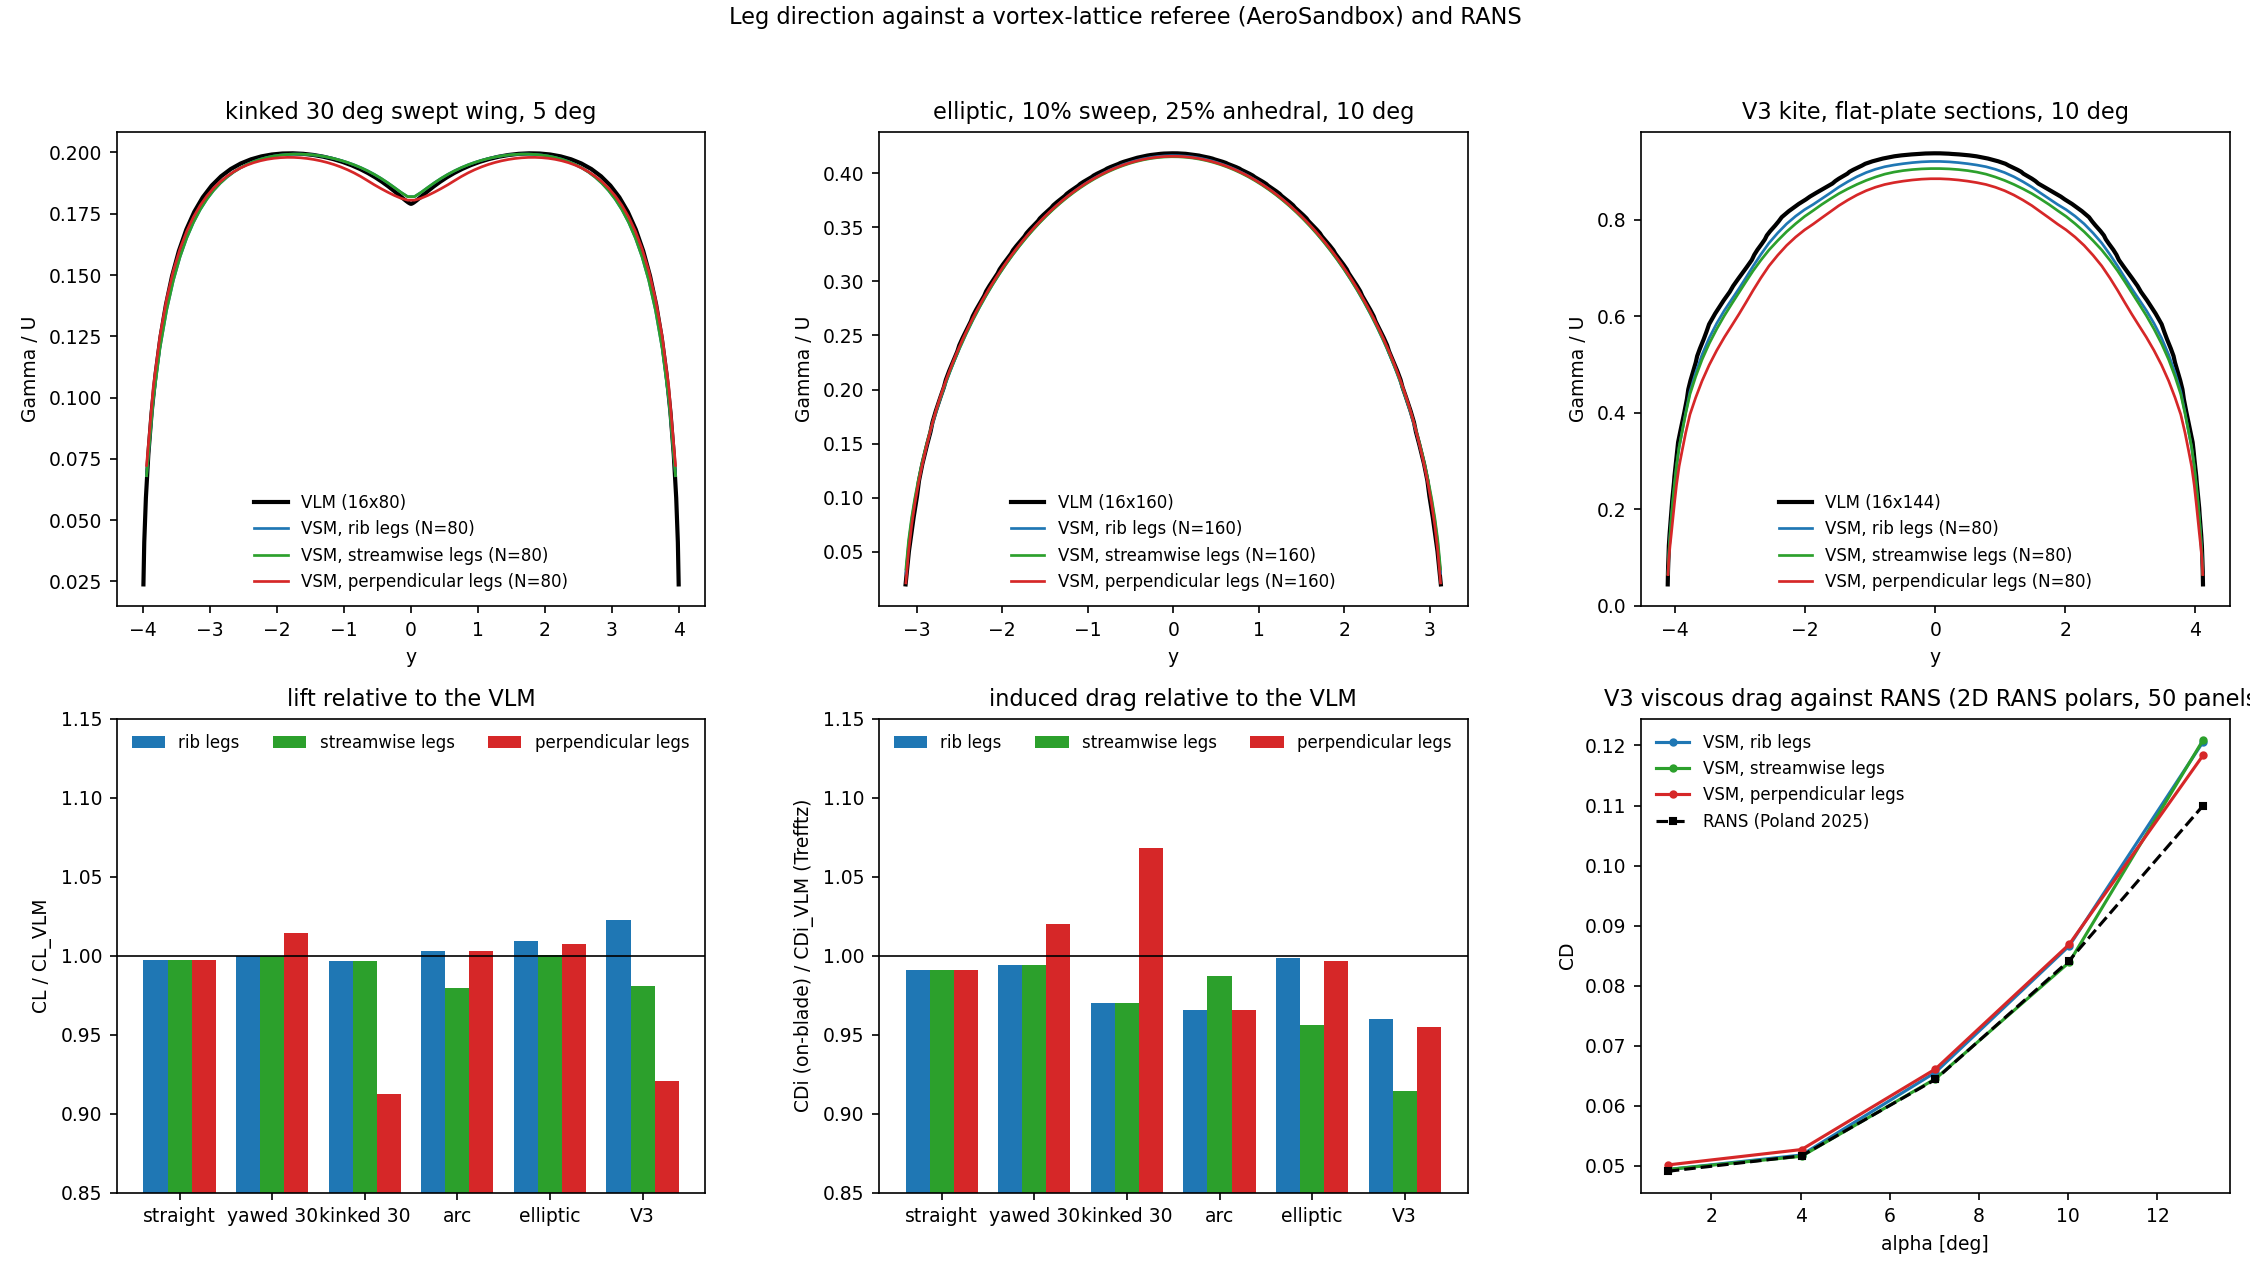
\includegraphics[width=\textwidth]{11_leg_direction_referee.png}
\caption{Vortex-lattice referee (\code{leg\_direction\_study.py --figures}). Top: strip circulation of the VLM and of the VSM with the three leg constructions. Bottom: lift and on-blade induced drag relative to the VLM, and the V3 viscous drag against RANS for the three constructions.}
\label{fig:referee}
\end{figure}

\begin{table}[t]\centering\small
\caption{VSM relative to the vortex-lattice referee: lift, and on-blade induced drag over the VLM's Trefftz drag (VSM at 80 panels, elliptic 160).}
\label{tab:referee}
\begin{tabular}{lcc|cc|cc|cc}
\toprule
 & \multicolumn{2}{c|}{VLM} & \multicolumn{2}{c|}{rib legs} & \multicolumn{2}{c|}{streamwise} & \multicolumn{2}{c}{perpendicular}\\
case & $C_L$ & $C_{D_i}$ & $C_L$ & $C_{D_i}$ & $C_L$ & $C_{D_i}$ & $C_L$ & $C_{D_i}$\\
\midrule
straight AR 8, $5^\circ$ & 0.402 & 0.00654 & $-0.2\,\%$ & $-0.9\,\%$ & $-0.2\,\%$ & $-0.9\,\%$ & $-0.2\,\%$ & $-0.9\,\%$\\
yawed $30^\circ$, $5^\circ$ & 0.360 & 0.00537 & $0.0\,\%$ & $-0.6\,\%$ & $0.0\,\%$ & $-0.6\,\%$ & $+1.4\,\%$ & $+2.0\,\%$\\
kinked swept $30^\circ$, $5^\circ$ & 0.363 & 0.00568 & $-0.4\,\%$ & $-3.0\,\%$ & $-0.4\,\%$ & $-3.0\,\%$ & $-8.8\,\%$ & $+6.7\,\%$\\
arc $110^\circ$, $8^\circ$ & 0.577 & 0.01481 & $+0.3\,\%$ & $-3.4\,\%$ & $-2.1\,\%$ & $-1.2\,\%$ & $+0.3\,\%$ & $-3.4\,\%$\\
elliptic, swept--anhedral, $10^\circ$ & 0.807 & 0.02643 & $+0.9\,\%$ & $-0.1\,\%$ & $+0.1\,\%$ & $-4.4\,\%$ & $+0.8\,\%$ & $-0.3\,\%$\\
V3, flat plate, $10^\circ$ (approx.) & 0.624 & 0.02961 & $+2.3\,\%$ & $-4.0\,\%$ & $-1.9\,\%$ & $-8.6\,\%$ & $-7.9\,\%$ & $-4.5\,\%$\\
\bottomrule
\end{tabular}
\end{table}

What the referee says: with rib legs the VSM reproduces the lifting-surface lift within $1\,\%$ on every wing except the V3 (2.3\,\%, where the referee itself is approximate) and the induced drag within 4\,\%; streamwise legs are equivalent on the planar wings and on the elliptic wing, 2\,\% low on the arc (the legs climb along the vertical tips) and closest to RANS on the V3; the paper's perpendicular legs lose 9\,\% of the lift on the kinked wing and 8\,\% on the V3, where they also cross at the tips above 80 panels, and are rejected. On the arc wing the rib legs stay within $+0.3$, $+1.6\,\%$ of the VLM lift at $8$ and $15^\circ$ while the streamwise legs drift to $-2.1$, $-3.0\,\%$. The lift distributions of the VLM and the VSM coincide along the span (Figure~\ref{fig:referee}, top), so the small differences in the totals are not local defects.

\subsection{The TU Delft V3 kite against RANS and the wind tunnel}
\label{sec:val-v3}
The V3 is a 25\,m$^2$ leading-edge inflatable kite with a strongly curved, swept planform. The VSM uses its CAD geometry with two-dimensional RANS polars of the rib sections at Re\,$5\times10^5$ (optionally NeuralFoil polars with transition), 50 panels, and is compared with the three-dimensional RANS of Poland et al.~\cite{poland2026} (Re\,$10^6$, no bridles) and with the wind-tunnel measurements of the same authors on a 1:6.5 rigid model without bridles (Re\,$5\times10^5$, support tare subtracted, open-jet correction applied). Table~\ref{tab:v3} and Figures~\ref{fig:v3polars} and~\ref{fig:v3before} give the comparison.

\begin{table}[t]\centering\small
\caption{V3 kite, zero sideslip, 50 panels, rib legs, 2D RANS polars: VSM against RANS (\code{leg\_direction\_study.py}) and the wind tunnel (\code{curved\_bound\_vortex\_validation.py}; the measured angles differ slightly from the nominal ones).}
\label{tab:v3}
\begin{tabular}{c|cc|cc|c}
\toprule
 & \multicolumn{2}{c|}{VSM} & \multicolumn{2}{c|}{RANS} & wind tunnel\\
$\alpha$ & $C_L$ & $C_D$ & $C_L$ & $C_D$ & $C_D$\\
\midrule
$1^\circ$ & 0.207 & 0.0494 & 0.228 & 0.0491 & --\\
$4^\circ$ & 0.461 & 0.0518 & 0.461 & 0.0517 & --\\
$5^\circ$ & -- & 0.055 & -- & 0.052 ($4^\circ$) & 0.076 ($5.4^\circ$)\\
$7^\circ$ & 0.697 & 0.0656 & 0.675 & 0.0644 & 0.090 ($7.3^\circ$)\\
$9^\circ$ & -- & 0.079 & -- & 0.084 ($10^\circ$) & 0.107 ($9.4^\circ$)\\
$10^\circ$ & 0.917 & 0.0866 & 0.869 & 0.0842 & --\\
$13^\circ$ & 1.050 & 0.1206 & 1.043 & 0.1100 & 0.217 ($13.4^\circ$)\\
\bottomrule
\end{tabular}
\end{table}

Against RANS the drag is within 3\,\% up to $10^\circ$ and 10\,\% high at $13^\circ$, near the RANS stall; the lift is within $0.02$ on average, with a lift slope of $0.078$ per degree against $0.067$ in RANS and the wind tunnel. The wind tunnel measures more drag than any simulation, RANS included: the gap is lift-dependent, $\Delta C_D\approx0.003+0.037\,C_L^2$, while the zero-lift drag agrees (wind tunnel 0.041, VSM 0.038, RANS 0.043). Poland et al.\ attribute it to the 3--4\,mm model canopy, the flow behind the leading-edge tube and transition. It is not a lifting-line issue; the three-quarter-chord force directions of the old code appeared to close part of it only because they overestimate the induced drag by 20--40\,\% (Figure~\ref{fig:v3before}), a compensating error. The physically defensible levers for the wind tunnel are two-dimensional polars with transition at the test Reynolds number ($+0.009$ in $C_D$ at $9.4^\circ$) and, for flight, the bridles.

\begin{figure}[p]\centering
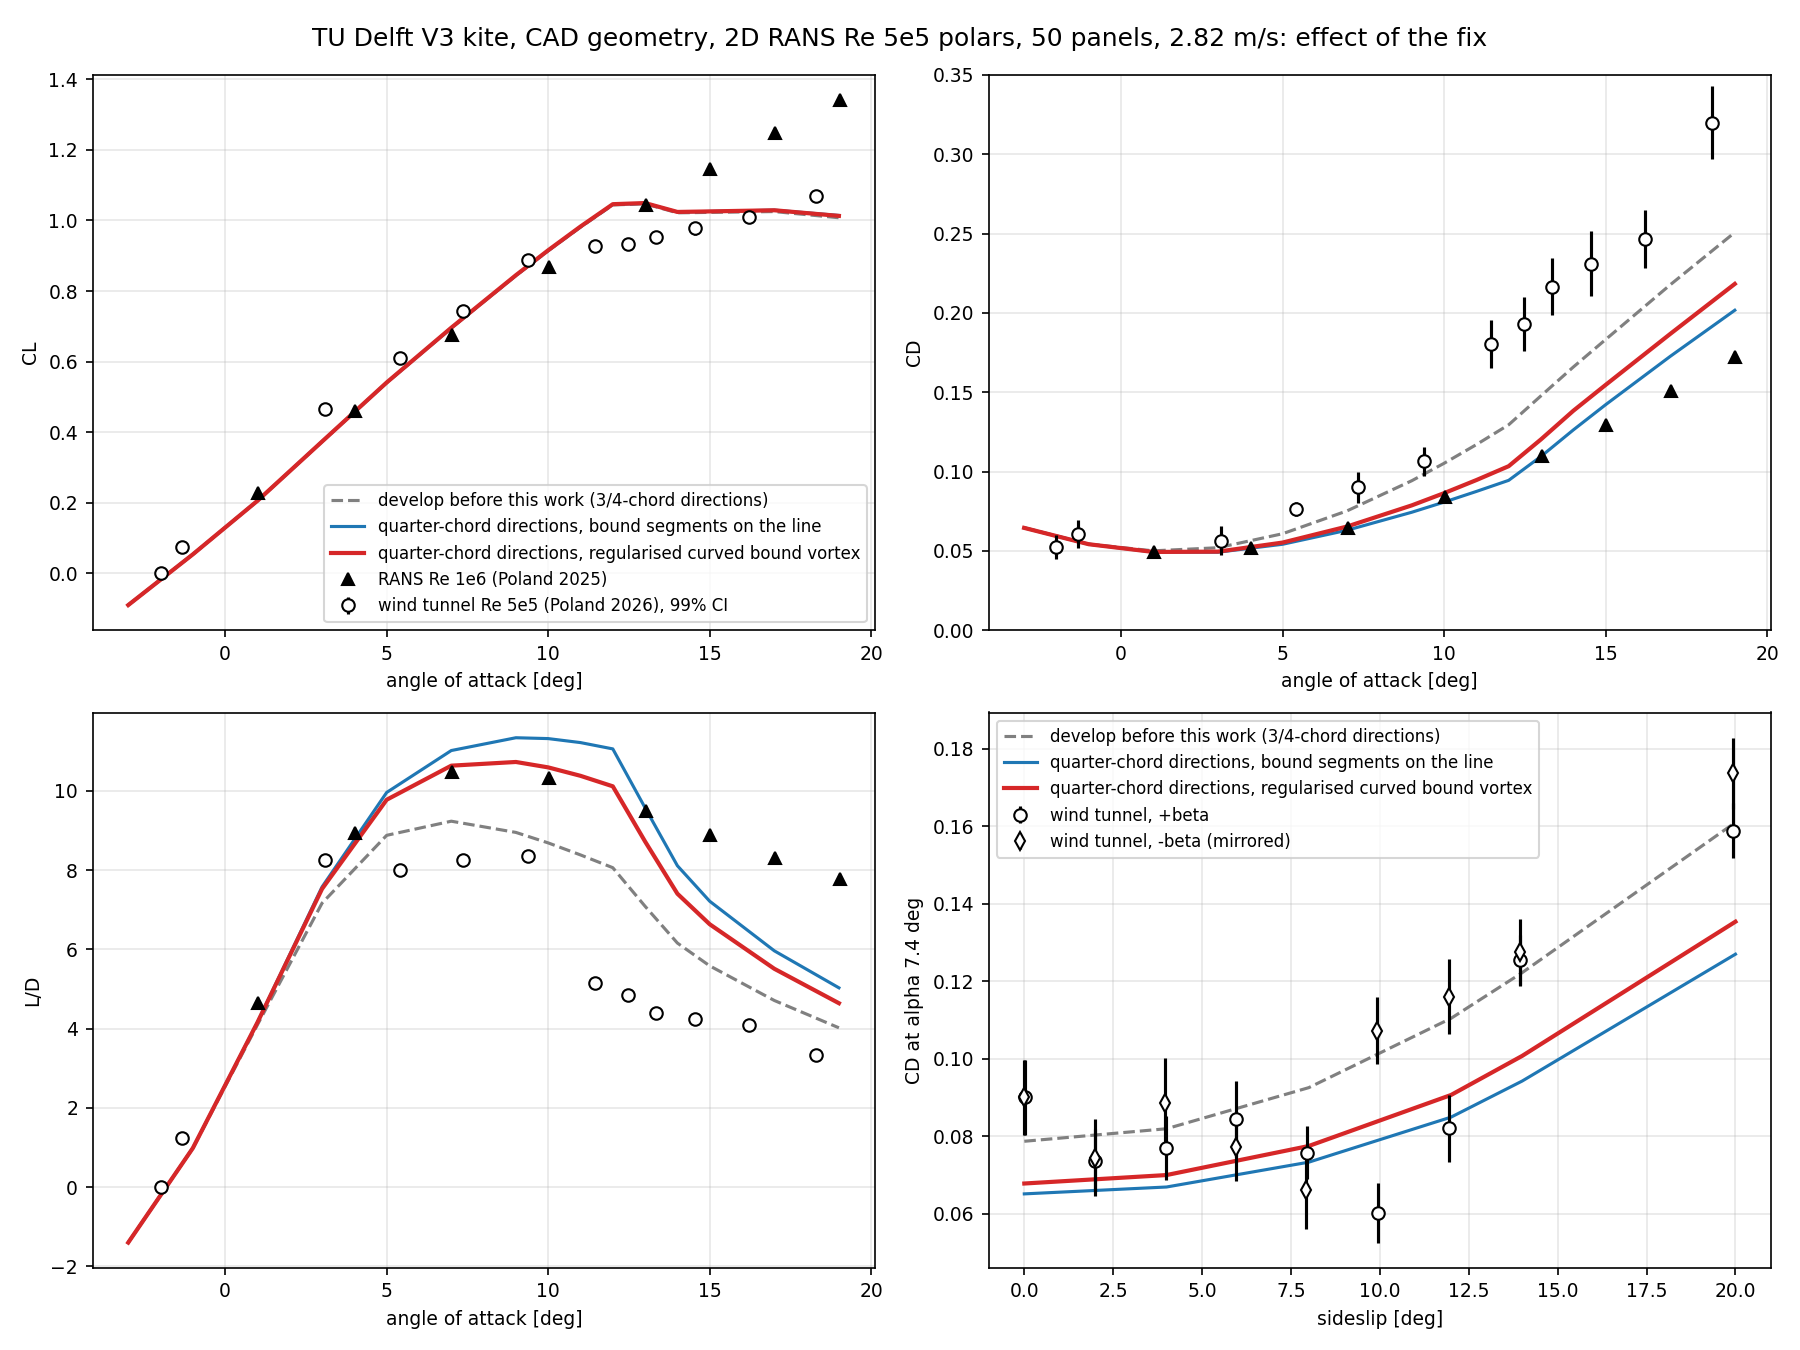
\includegraphics[width=\textwidth]{09_v3_polars_curved_bound_vortex_fix.png}
\caption{V3 polars (\code{curved\_bound\_vortex\_validation.py --figures}): the solver before the consistent coupling (grey dashed), quarter-chord directions with the singular bound-on-line term (blue) and with the regularisation (red), against RANS and the wind tunnel.}
\label{fig:v3polars}
\end{figure}

\begin{figure}[p]\centering
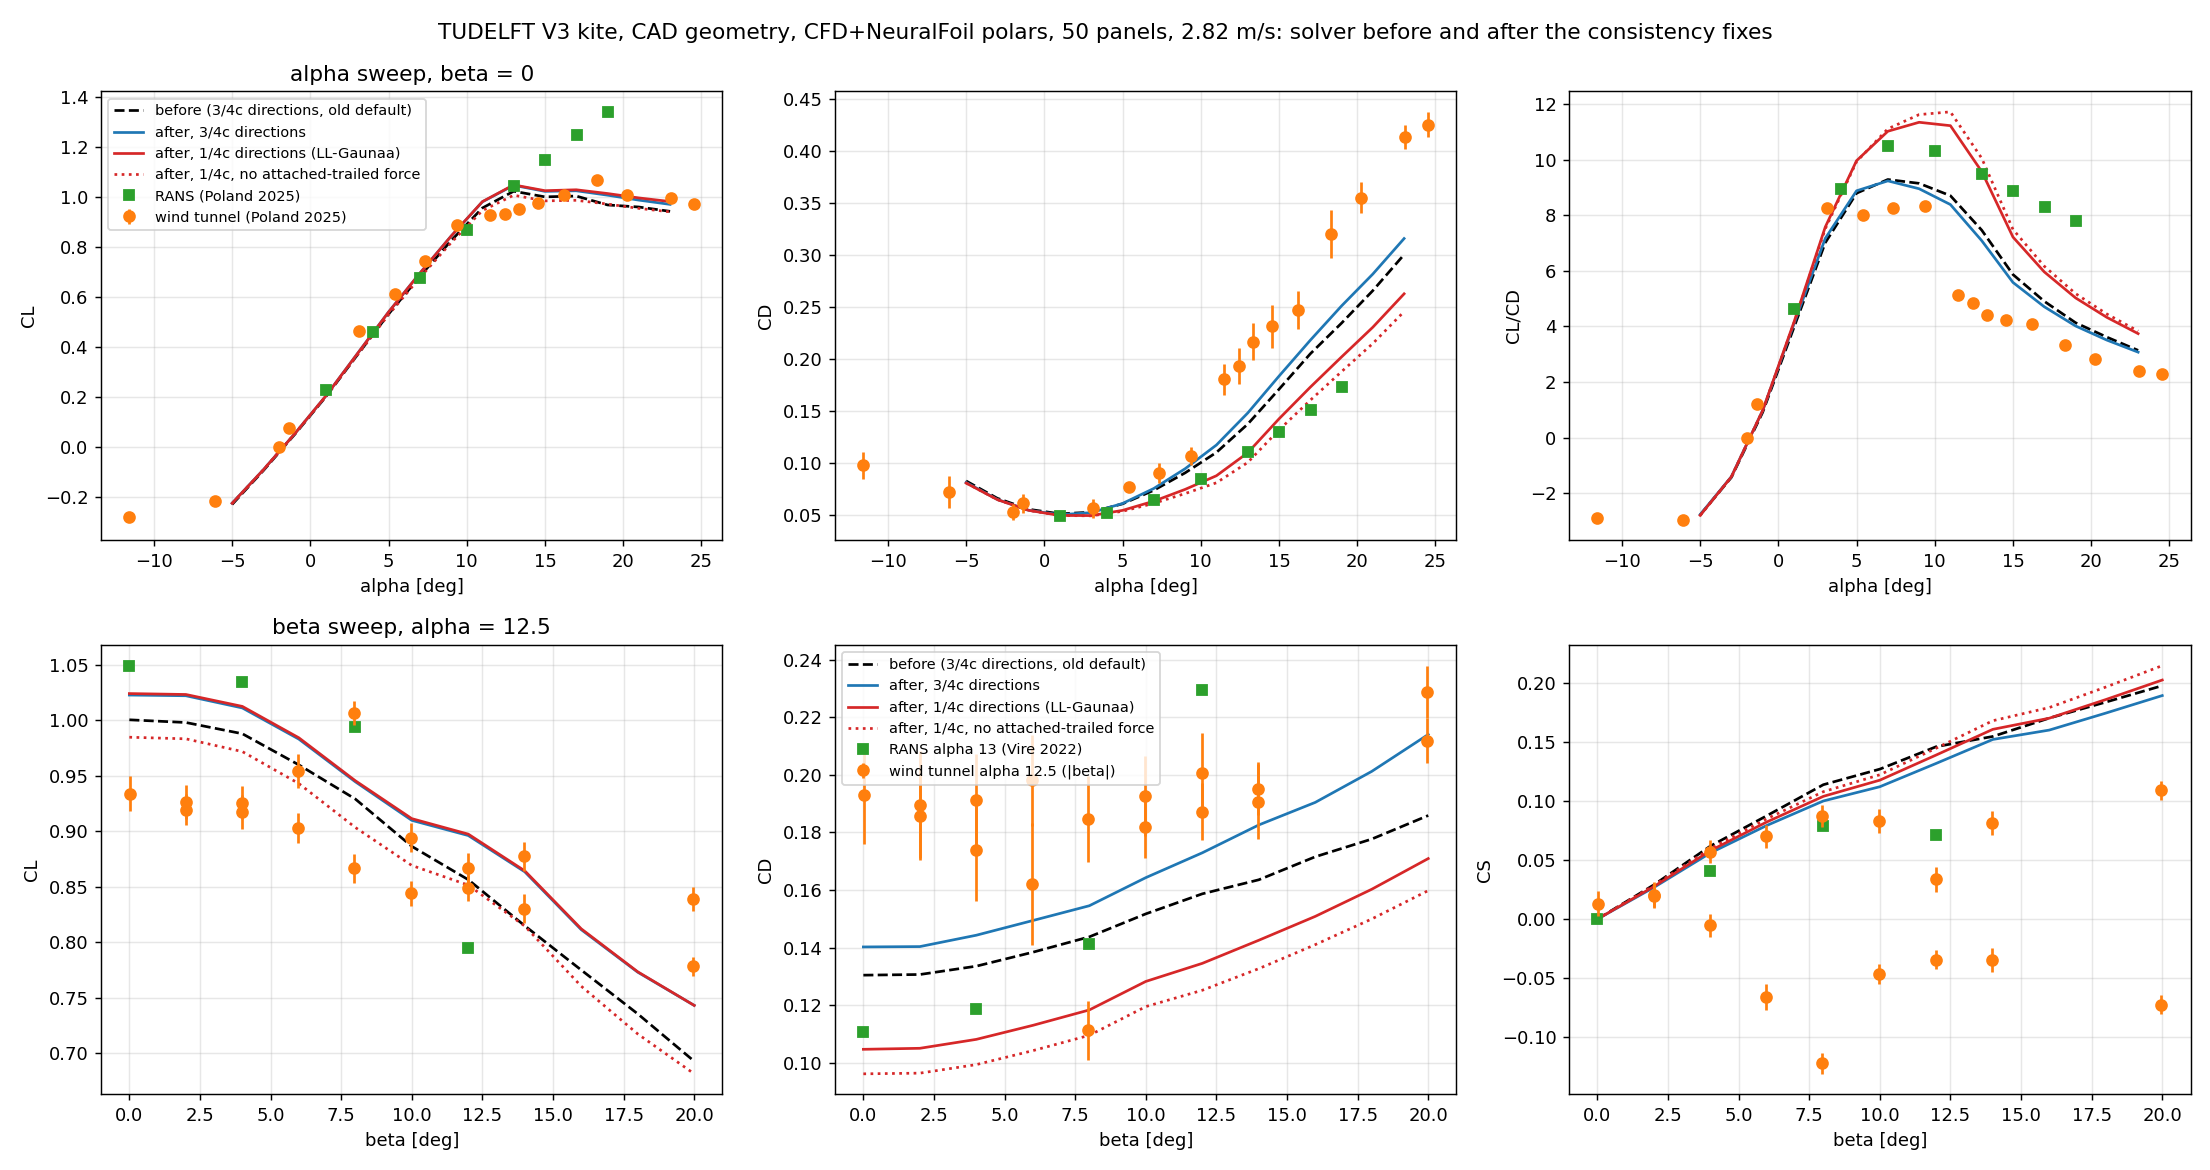
\includegraphics[width=\textwidth]{01_v3_polars_before_after.png}
\caption{V3 polars before and after the consistent coupling (\code{make\_pr\_figures.py}): the old solver (dashed black), the consistent implementation with three-quarter-chord directions (blue) and with quarter-chord directions (red, the default), dotted without the attached-trailed force, against RANS and wind-tunnel data, including sideslip.}
\label{fig:v3before}
\end{figure}

\subsection{Mesh convergence}
\label{sec:val-mesh}
Figure~\ref{fig:mesh} shows lift, induced drag and the on-blade over Trefftz ratio of the inviscid V3 and of the straight wing against the number of panels, 10 to 160, uniform spacing. On the V3 the lift is within $0.4\,\%$ of its 160-panel value from 10 panels on and the induced drag within $3\,\%$ (within $0.5\,\%$ from 40 panels), with the on-blade over Trefftz ratio between 1.007 and 1.021. On the straight wing the lift converges from above ($5\,\%$ high at 10 panels, $1\,\%$ at 40), because the tip loading needs panels to be resolved, the induced drag is within $1.3\,\%$ throughout, and the ratio is 1.000 at every count. Fifty panels, the usual choice for the V3, put every integral quantity within $1\,\%$ of the converged value.

\begin{figure}[t]\centering
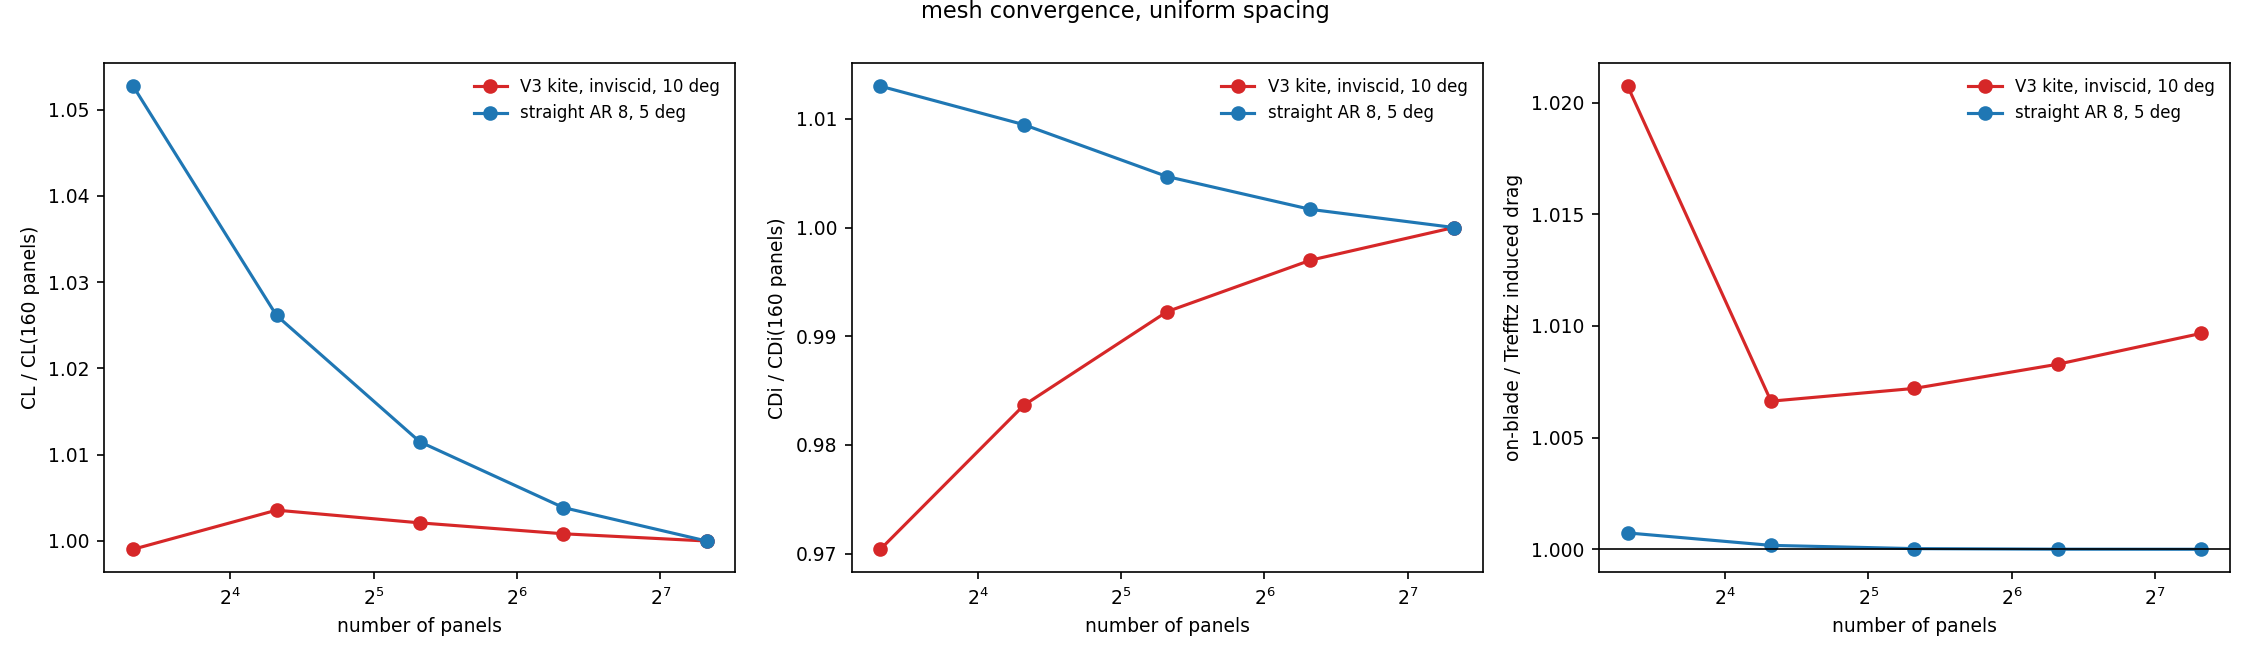
\includegraphics[width=\textwidth]{13_mesh_convergence.png}
\caption{Mesh convergence (\code{aerodynamic\_model\_figures.py}): lift and induced drag relative to the 160-panel value, and the on-blade over Trefftz ratio, for the inviscid V3 at $10^\circ$ and the straight AR 8 wing at $5^\circ$.}
\label{fig:mesh}
\end{figure}

\subsection{Regression cases in the test suite}
\label{sec:val-tests}
The test suite (\code{pytest tests}, 182 tests) holds, besides unit tests of every module: the analytical horseshoe case; the elliptic wing against Prandtl; a curved wing of aspect ratio 3.2 and a $30^\circ$ swept wing against the thesis implementation and, for the swept wing, XFLR5 and CFD polars; the V3 against the thesis implementation and the RANS polars; the Trefftz consistency of the regularisation on the arc wing at 20, 40 and 80 panels; the leg constructions (equality where they must coincide, the skewed-rib invariance, the kinked wing, the sideslip rebuild, the pure-rotation fallback); the relaxation-factor bound; body rates and distributed inflow; and the wake direction. The cases that verify the thesis vortex system pass \code{leg\_direction="rib"} explicitly.

\subsection{Limits of the model}
\label{sec:limits}
The model is a steady, attached-flow, thin-surface method. It does not capture: stall and post-stall flow beyond what the sectional polars and the artificial viscosity provide; wake roll-up and the interaction of the wake with downstream surfaces; unsteady effects (shed vorticity, added mass); thickness effects on the induced flow; and the viscous drag sources that the V3 wind tunnel sees beyond RANS. On curved wings the on-blade induced drag carries a few per cent of uncertainty with respect to a lifting-surface solution, and the lift slope of the V3 is 15\,\% steeper than measured. The direction of the attached-trailed legs is a modelling choice; the rib construction is the default and the streamwise one the alternative for uniform inflow (Section~\ref{sec:val-legs}).

\section{Conventions}
\label{sec:conventions}
\begin{table}[h]\centering\small
\begin{tabular}{>{\raggedright\arraybackslash}p{0.28\textwidth}>{\raggedright\arraybackslash}p{0.66\textwidth}}
\toprule
item & convention\\
\midrule
global frame & right-handed; kite data and examples: $x$ downstream, $y$ to the left tip, $z$ up\\
panel frame & $\vect e_s$ (\code{z\_airf}) along the bound vortex towards the left tip; $\vect e_c$ (\code{y\_airf}) leading to trailing edge, perpendicular to the span; $\vect e_n$ (\code{x\_airf}) $=\vect e_c\times\vect e_s$, suction side\\
chord & perpendicular to the local quarter-chord line (CP1), averaged over the panel's two sections\\
bound vortex, control point & at $1/4$ and $3/4$ of the chord by default (\code{aerodynamic\_center\_location}, \code{control\_point\_location})\\
circulation & positive for positive lift in the panel frame; ring sense bound $\vect b_2\to\vect b_1$, leg $\vect b_1\to\vect T_1$, leg $\vect T_2\to\vect b_2$\\
angle of attack, sideslip & degrees in \code{va\_initialize}; $\vect V_a=U(\cos\alpha\cos\beta,\ \sin\beta,\ \sin\alpha\cos\beta)$ in the global frame\\
body rates & about given axes through \code{reference\_point}; $\vect V_{a,i}=\vect V_\infty-\boldsymbol\omega\times(\vect C_i-\vect r_0)$\\
polars & $[\alpha\ \text{(rad)},\ C_l,\ C_d,\ C_m]$, $C_m$ about the quarter chord\\
lift, drag, side & along $\vect V_{\mathrm{ref}}\times\vect e_{\mathrm{span}}$, $\vect V_{\mathrm{ref}}$ and their cross product; coefficients on $q_{\mathrm{ref}}$ and the projected area\\
moments & about \code{reference\_point}, coefficients on projected area times largest chord\\
units & SI throughout; $\rho=1.225$\,kg/m$^3$, $\mu=1.81\times10^{-5}$\,Pa\,s by default\\
\bottomrule
\end{tabular}
\end{table}

\begin{thebibliography}{99}\small
\bibitem{gaunaa2026} M.~Gaunaa, A.~Li, G.~R.~Pirrung, From thin airfoil theory to finite wings: consistent implementation of Lifting Line-based models, J.\ Phys.: Conf.\ Ser.\ 3224 (2026) 042030.
\bibitem{li2026} A.~Li, M.~Gaunaa, G.~R.~Pirrung, K.~L{\o}nb{\ae}k, Relaxation limits and artificial viscosity for lifting line methods, TORQUE 2026.
\bibitem{li2020} A.~Li, M.~Gaunaa, G.~R.~Pirrung, N.~Ramos-Garc\'ia, S.~G.~Horcas, The influence of the bound vortex on the aerodynamics of curved wind turbine blades, J.\ Phys.: Conf.\ Ser.\ 1618 (2020) 052038.
\bibitem{gaunaa2024} M.~Gaunaa, N.~N.~S{\o}rensen, A.~Li, Spanwise-flow correction of the viscous forces in lifting-line methods, J.\ Phys.: Conf.\ Ser.\ 2767 (2024) 022068.
\bibitem{reid2020} J.~T.~Reid, D.~F.~Hunsaker, A general approach to lifting-line theory, applied to wings with sweep, J.\ Aircraft 58 (2021), doi:10.2514/1.C035994.
\bibitem{damiani2019} R.~Damiani, F.~F.~Wendt, J.~M.~Jonkman, J.~Sicard, A vortex step method for nonlinear airfoil polar data as implemented in KiteAeroDyn, AIAA SciTech 2019, paper 2019-0804.
\bibitem{poland2026} J.~A.~W.~Poland, J.~M.~van Spronsen, M.~Gaunaa, R.~Schmehl, Wind tunnel load measurements of a leading-edge inflatable kite rigid-scale model, Wind Energ.\ Sci.\ 11 (2026) 911.
\bibitem{aerosandbox} P.~D.~Sharpe, AeroSandbox: a differentiable framework for aircraft design optimization, MIT (2021), \url{https://github.com/peterdsharpe/AeroSandbox}; version 4.2.8, \code{VortexLatticeMethod}.
\bibitem{report} Vortex-Step-Method repository, The curved bound vortex at the quarter chord of a lifting line: problem, regularisation, literature and the direction of the attached-trailed legs, \code{docs/validation/curved\_bound\_vortex\_report.pdf} (2026).
\bibitem{cayon2022} O.~Cayon, Fast aeroelastic model of a leading-edge inflatable kite, MSc thesis, TU Delft (2022); its chapter~4 was the previous content of this document.
\end{thebibliography}

\end{document}
